% options:
% thesis=B bachelor's thesis
% thesis=M master's thesis
% czech thesis in Czech language
% slovak thesis in Slovak language
% english thesis in English language
% hidelinks remove colour boxes around hyperlinks

\documentclass[thesis=M,czech]{FITthesis}[2012/06/26]

\usepackage[utf8]{inputenc} % LaTeX source encoded as UTF-8

\usepackage{graphicx} %graphics files inclusion
% \usepackage{amsmath} %advanced maths
% \usepackage{amssymb} %additional math symbols

\usepackage{dirtree} %directory tree visualisation

%Moje packages%%%%%%%%%%%%%%%%%%%%%%%%%%%%%%%%%%%%%
\usepackage{todonotes}
\usepackage{multirow}
\usepackage{hyperref}
\usepackage{enumitem}

% % list of acronyms
\usepackage[acronym,nonumberlist,toc,numberedsection=autolabel]{glossaries}
\iflanguage{czech}{\renewcommand*{\acronymname}{Seznam pou{\v z}it{\' y}ch zkratek}}{}
\makeglossaries

\newcommand{\tg}{\mathop{\mathrm{tg}}} %cesky tangens
\newcommand{\cotg}{\mathop{\mathrm{cotg}}} %cesky cotangens

% % % % % % % % % % % % % % % % % % % % % % % % % % % % % % 
% ODTUD DAL VSE ZMENTE
% % % % % % % % % % % % % % % % % % % % % % % % % % % % % % 

\department{Katedra softwarového inženýrství}
\title{Využití konceptu BYOD a jeho zabezpečení v bankovním prostředí}
\authorGN{Vojtěch} %(křestní) jméno (jména) autora
\authorFN{Dlápal} %příjmení autora
\authorWithDegrees{Bc. Vojtěch Dlápal} %jméno autora včetně současných akademických titulů
\supervisor{Ing. Pavel Krejčí}
\acknowledgements{Doplňte, máte-li komu a za co děkovat. V~opačném případě úplně odstraňte tento příkaz.}
\abstractCS{V~několika větách shrňte obsah a přínos této práce v~češtině. Po přečtení abstraktu by se čtenář měl mít čtenář dost informací pro rozhodnutí, zda chce Vaši práci číst.}
\abstractEN{Sem doplňte ekvivalent abstraktu Vaší práce v~angličtině.}
\placeForDeclarationOfAuthenticity{V~Praze}
\declarationOfAuthenticityOption{4} %volba Prohlášení (číslo 1-6)
\keywordsCS{Nahraďte seznamem klíčových slov v češtině oddělených čárkou.}
\keywordsEN{Nahraďte seznamem klíčových slov v angličtině oddělených čárkou.}

\begin{document}

\todo{doplnit podekovani}
\todo{napsat abstrakt}
\todo{prelozit abstrakt}
\todo{klicova slova}

% \newacronym{CVUT}{{\v C}VUT}{{\v C}esk{\' e} vysok{\' e} u{\v c}en{\' i} technick{\' e} v Praze}
% \newacronym{FIT}{FIT}{Fakulta informa{\v c}n{\' i}ch technologi{\' i}}


%%%%%%%%%%%%%%%%%%%%%%%%%%%%%%%%%%%%%%%%%%%%%%%%%%%%%%%%%%%%%%%%%%%%%%%%%%%%%%%%%%%
%%%%%%%%%%%%%%%%%%%%%%   ZADANI    %%%%%%%%%%%%%%%%%%%%%%%%%%%%%%%%%%%%%%%%%%%%%%%%
%%%%%%%%%%%%%%%%%%%%%%%%%%%%%%%%%%%%%%%%%%%%%%%%%%%%%%%%%%%%%%%%%%%%%%%%%%%%%%%%%%%

%Definujte klíčové faktory a rizika využití BYOD v bankovním prostředí.

%Analyzujte dostupná existující řešení BYOD, zejména z pohledu bezpečnosti.

%Ve vybrané bankovní organizaci analyzujte požadavky na připojení vlastních zařízení a identifikujte hlavní hrozby související s nasazením BYOD.

%Analyzujte stávající bezpečností procesy v připojování nefiremních zařízení do její vnitřní sítě.

%Vyberte nejvhodnější variantu na trhu dostupného řešení a konfrontujte ji s praxí ve vybrané organizaci. 

%Konzultujte navrhované řešení se zástupci vybrané organizace a stanovte doporučení pro nasazení. 

%Navrhněte nasazení řešení BYOD. 

%Zhodnoťte uskutečnitelnost řešení a analyzujte benefity a rizika spojená se zavedením navrženého konceptu.

\listoftodos[Co je treba udelat]
%%%%%%%%%%%%%%%%%%%%%%%%%%%%%%%%%%%%%%%%%%%%%%%%%%%%%%%%%%%%%%%%%%%%%%%%%%%%%%%%%%%
%%%%%%%%%%%%%%%%%%%%%%%%%%%%%%%%%%%%%%%%%%%%%%%%%%%%%%%%%%%%%%%%%%%%%%%%%%%%%%%%%%%
%%%%%%%%%%%%%%%%%%%%%%%%%%%%%%%%%%%%%%%%%%%%%%%%%%%%%%%%%%%%%%%%%%%%%%%%%%%%%%%%%%%
% --------------->>>> TEXT PRACE <<<<<<<------------------------------%
%%%%%%%%%%%%%%%%%%%%%%%%%%%%%%%%%%%%%%%%%%%%%%%%%%%%%%%%%%%%%%%%%%%%%%%

\begin{introduction}
	%sem napište úvod Vaší práce
	\section{Cíl práce}
Cílem této práce bylo zhodnotit koncept BYOD a jeho využití v bankovním prostředí. Analýza probíhala ve vybrané bankovní organizaci, požadavkem bylo najít vhodné řešení pro BYOD a to především s důrazem na bezpečnost.

Tato práce probíhala v úzké spolupráci s vybranou bankovní organizaci a to formou schůzek a konzultací zprostředkovaných oddělením IT Security. Práce odpovídá na otázky co to BYOD je, co vede společnosti k úvahám o tomto konceptu a jaké jsou možnosti řešení.  Na základě analýzy vybrané bankovní organizace vybírá nejvhodnější řešení na aktuálním trhu a stanovuje doporučení pro jejich nasazení ve vybrané organizaci. Navržené řešení je vyhodnoceno na základě benefitů a rizik spojených se zavedením a zpětné vazby od vybrané organizace.

%%% COPY PASTE %%%%
\ref{k1}\todo{odcopypastovat}
Tato kapitola je zaměřena na BYOD jako termín. Definuje jej s použitím několika zdrojů a uvádí jej do kontextu s aktuální situací v České republice i zahraničí. Zmiňuje důvody, proč je vhodné, aby se firmy problematikou zabývaly. Dále rozvádí obecně známe benefity a hrozby zavedení konceptu do firem. Závěr kapitoly se zabývá podněty nutnými ke zvážení z hlediska firemních politik, právního prostředí a především aktuální situace z hlediska kybernetické bezpečnosti.  

%%% COPY PASTE %%%%
\ref{k2}\todo{odcopypastovat}
Tato kapitola seznamuje čtenáře s výsledky analýzy vybrané bankovní organizace. Nejdříve je organizace krátce představena a jsou vyjmenována některá specifika tohoto typu organizací. Dále je podrobně analyzován stávající proces připojování nefiremních zařízení do firemní sítě včetně použitých technických prostředků a tento proces je dále podroben analýze souvisejících hrozeb. V neposlední řadě jsou analyzovány známé požadavky na BYOD dané organizaci a typické skupiny uživatelů a jejich potřeb. Závěr kapitoly se zabývá dříve uskutečněnými projekty v organizaci dotýkající se problematiky BYOD.

\todo{napsat úvod}
\end{introduction}

\chapter{Charakteristika BYOD}\label{k1}
%Definujte klíčové faktory a rizika využití BYOD v bankovním prostředí.

\section{Trendy v ICT pro spotřebitele}\label{trendy} \todo{nejake statistiky a magic quadranty}

Podle ředitele odboru statistik a rozvoje Českého statistického úřadu Martina Mana \textit{Je zajímavé, že počet uživatelů internetu převyšuje počet uživatelů počítače. Je to dáno hlavně rozmachem chytrých telefonů a jiných přenosných zařízení, která jsou častěji využívána i k přístupu na internet. Lze předpokládat, že internet se ve spojení s mobilem brzy stane široce rozšířenou technologií používanou napříč všemi věkovými a vzdělanostními  kategoriemi,} \todo{citace https://www.czso.cz/csu/czso/chytre-telefony-zvysuji-pocet-uzivatelu-internetu}. Podle předsedkyně Českého statistického úřadu Ivy Ritschelové v citátu z května 2016 \textit{Až do roku 2013 dominovaly českým domácnostem klasické stolní počítače. Vloni je vystřídaly počítače přenosné. Mělo je 55 \% všech domácností, resp. 75 \% domácností, které jsou vybaveny počítačem}.

Podle výzkumu provedeným společností TNS Infratest pro společnost Google vlastnilo v roce 2016 v České republice chytrý telefon připojený k internetu 50 \% všech obyvatel. \todo{https://www.consumerbarometer.com/en/about/}  To je oproti 17 \% z roku 2012 drastický nárůst a je možné pozorovat dále vzrůstající trend \ref{uzivateleSmartphone}. Dále zřejmé, že trend v České republice bude dále dohánět rozšíření chytrých mobilních telefonů v technologicky vyspělejších zemích jako jsou Spojené státy, nebo sousední Německo. Ve Spojených státech dosáhla adopce chytrých mobilních v roce 2016 72 \%.

\begin{figure}[h!]\label{uzivateleSmartphone}
\centering
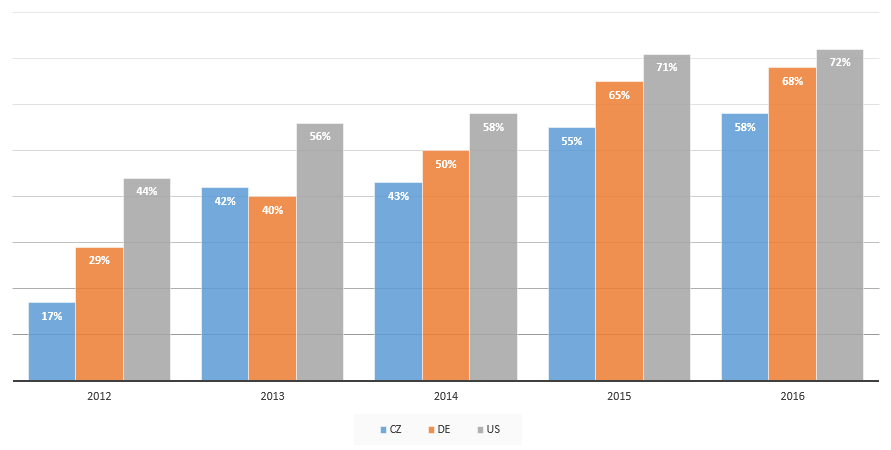
\includegraphics[width=13cm]{img/uzivateleSmartphone}
\caption{Poměrná část uživatelů chytrých telefonů k celé populaci v České republice, Německu a spojených státech. Zdroj: } 
\end{figure}\todo{citovat }

Jiným typem zařízení, které zaznamenávají zvýšenou popularity jsou tablety. V roce 2012 vlastnilo v České republice tablet připojený k internetu 4 \% obyvatelstva. V roce 2016 to bylo již 26 \% což je více než šestinásobek uživatelů v rozmezí ctyř let. V USA vlastní tablet připojený k internetu dokonce 42 \% obyvatelstva a trend je nadále stoupající. 

\begin{figure}[h!]\label{uzivateleTablet}
\centering
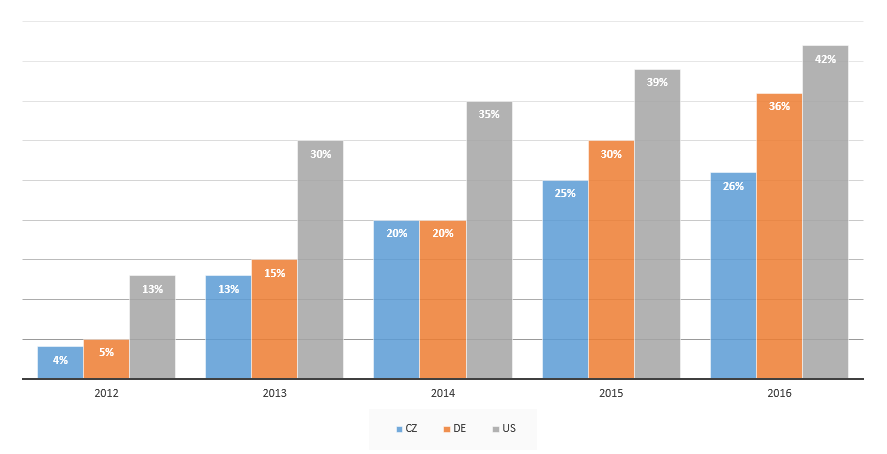
\includegraphics[width=13cm]{img/uzivateleTablet}
\caption{Poměrná část uživatelů tabletů k celé populaci v České republice, Německu a spojených státech. Zdroj: } 
\end{figure}\todo{citovat }

Další zajímavou statistikou je průměrný počet zařízení připojených k síti internet na jednoho obyvatele daného státu v daném státě. V roce 2012 obyvatel České republiky vlastnil v průměru 1,6 zařízení, zatímco v roce 2016 to bylo 2,5. Průměrný Američan vlastnil v roce 2016 3.5 zařízení připojených k internetu. To znamená nejspíše počítač, chytrý telefon, tablet a další zařízení.

\begin{figure}[h!]\label{pocetZarizeni}
\centering
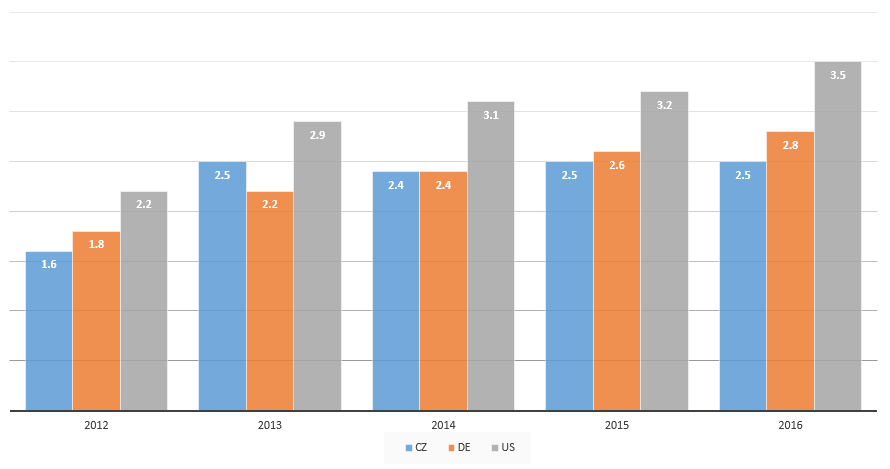
\includegraphics[width=13cm]{img/pocetZarizeni}
\caption{Průměrný počet zařízení připojených k internetu na obyvatele v České republice, Německu a Spojených státech. Zdroj: } 
\end{figure}\todo{citovat }

Tato čísla ukazují, že počet obyvatel vlastnících zařízení z oblasti informačních a komunikačních technologií v posledních letech dramaticky roste. Lidé vlastnící své soukromé zařízení si vytvářejí návyky a začínají upřednostňovat některé technologie nad jinými.

Své návyky s obsluhou ICT ve svém soukromém životě by tak někteří zaměstnanci rádi začali uplatňovat i v životě pracovním. To může přinést jak zaměstnanci tak zaměstnavateli mnohé výhody, ale zároveň mnohá úskalí, se kterými je třeba se vyrovnat. Nastolená praxe, kdy zaměstnanec používá své vlastní zařízení k pracovním účelům, se souhrnně označuje termínem BYOD.



\section{Charakteristika BYOD}

BYOD je zkratka v anglickém jazyce znamenající "Bring your own device". Oxfordský slovník jej vysvětluje jako postup vedoucí k umožnění zaměstnancům organizace používat jejich vlastní počítače, chytré telefony a další zařízení k pracovním účelům. \todo{https://en.oxforddictionaries.com/definition/BYOD} 

Slovník Cambridge definuje BYOD jako postup firem nebo škol, který říká, že zaměstnanci nebo studenti si mohou přinést své vlastní počítače, telefony, atd.  do práce nebo školy za účelem jejich využití k práci. \todo{citace http://dictionary.cambridge.org/dictionary/english/byod}

Poradenská společnost Gartner BYOD definuje jako \textit{alternativní strategii povolující zaměstnancům, obchodním partnerům a dalším uživatelům používání osobně zvolených a zakoupených koncových zařízení ke spouštění podnikových aplikací a přístupu k datům. To typicky znamená chytré telefony a tablety, ale tato strategie může být také použita pro osobní počítače. Může obsahovat i finanční kompenzace.}

Konzultační společnost Deloitte definuje BYOD jako použití zařízení vlastněných zaměstnancem pro přístup k přístupu k podnikovému obsahu nebo sítím. \todo{citace https://www2.deloitte.com/content/dam/Deloitte/uk/Documents/about-deloitte/deloitte-uk-understanding-the-bring-your-own-device\%20landscape.pdf} Dále dále upřesňuje ve třech kategoriích a to zařízení, schopnosti a charakteristika. 

Zařízeníje specifikované jako vybavené procesorem a to specificky chytré telefony, tablety nebo počítače. Schopnosti se mohou lišit od pouhého přístupu k internetu skrze firemní síť po přístup k podnikovým aplikacím a systémům. Charakteristiou BYOD může být používání vlastních zařízení jako doplněk k firemním zařízením, jako náhradu firemního zařízení, nebo povolení k užití zařízení, které firma není zaměstnanci ochotna zajistit vlastními zdroji. 

Podle dat ze služby Google Analytics \todo{citace} se výraz BYOD začal rozšiřovat začátkem roku 2012. Graf \ref{hledaniBYOD} ukazuje popularitu vyhledávání výrazu BYOD za použití vyhledávače Google v čase vztažené relativně k období, kdy byl zadaný výraz vyhledáván nejčastěji. Je zřejmé, že zájem o tuto problematiku nepolevuje.

\begin{figure}[h!]\label{hledaniBYOD}
\centering
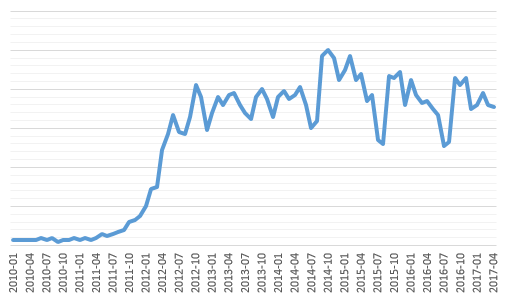
\includegraphics[width=13cm]{img/hledaniBYOD}
\caption{Relativní popularita vyhledávání termínu BYOD vztažená k maximální popularitě v daném období podle Google Analytics Zdroj: www.analytics.google.com } 
\end{figure}\todo{citovat }
 

Článek \todo{citovat consumeration} zmiňuje mnohé výhody modelu, kdy zaměstnanci používají svá vlastní zařízení jako například zvýšenou flexibilitu a produktivitu zaměstnanců. Dále zmiňuje snížení nákladů na technickou podporu zařízení, jelikož za svá zařízení si zaměstnanci odpovídají sami.

Na druhou stranu článek zmiňuje nutnost zavedení omezujících pravidel, jelikož nefiremní zařízení s sebou přinášejí řadu hrozeb jako jsou úniky dat či napadení firemní infrastruktury škodlivým software.  Další zmíněné negativum osobních zařízení ve firemním prostředí je nebezpečí využívání pracovní doby k soukromým účelům jako je hraní her, streamování videí a dalším činnostem snižujícím pracovní morálku.

Vzhledem k masovému rozšíření informačních technologií mezi spotřebiteli se stává pro firmy nutností zaujmout k soukromým zařízením jednoznačný postoj. BYOD zařízení ve firemním již nejsou pouze možností, ale každodenní realitou.

V době, kdy mnozí zaměstnanci vlastní výkonné chytré telefony, tablety, či dokonce nositelnosti a vnášejí je do firemního prostředí je nutné nastavit jasná pravidla, aby byla chráněna firemní infrastruktura a data.

Podle Pavla Housera z Hospodářských novin \todo{citovat http://ictrevue.ihned.cz/c3-65260640-0ICT00\_d-65260640-byod-prinasi-firmam-vyssi-produktivitu-i-bezpecnostni-rizika} již BYOD do firem prorostlo a stalo se realitou i přes snahu některých firem o zákaz. Autor tvrdí, že na konceptu BYOD vydělaly především firmy, které jej pochopily nejen jako hrozbu, ale i příležitost. 

Naopak podle tiskové zprávy společnosti Intel publikované v Hospodářských novinách \todo{ citace http://ictrevue.ihned.cz/c3-65456950-0ICT00\_d-65456950-byod-po-cesku-pouze-v-7-firem-vita-vyuziti-soukromych-pocitacu-zamestnancu} vítá koncept BYOD pouze 7 \% českých firem, zbytek se k tématu staví odměřeně. Respondenti jejího průzkumu mají výhrady především k bezpečnosti, viz \ref{intelBYOD}.

\begin{figure}[h!]\label{intelBYOD}
\centering
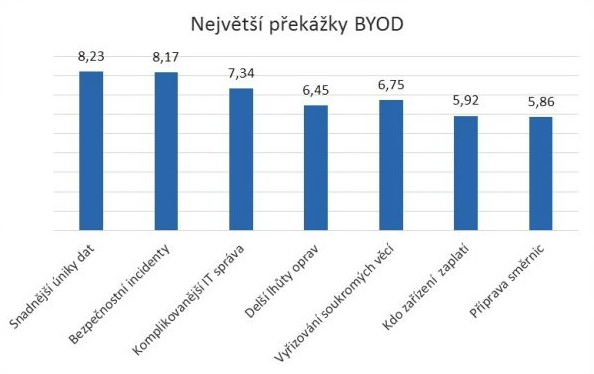
\includegraphics[width=12cm]{img/intelBYOD}
\caption{Největší negativa BYOD podle průzkumu společnosti Intel ohodnocené ve škále 1 až 10. Zdroj: } 
\end{figure}\todo{citovat http://ictrevue.ihned.cz/c3-65456950-0ICT00\_d-65456950-byod-po-cesku-pouze-v-7-firem-vita-vyuziti-soukromych-pocitacu-zamestnancu }

Společnost Deloitte ve svém článku uvádí tři možné přístupy k BYOD. Tolerovaní, zákaz nebo řízený BYOD program. Zatímco zákaz s sebou nese vysoké riziko nerespektování zaměstnanci a tím pádem i riziko bezpečnostní, řízený BYOD s sebou nese náklady na přípravu, zaškolení a provoz.

Jako hlavní výhody uvádí:
\begin{itemize}
\item Snížení nákladů na IT
\item Zvýšení produktivity
\item Zvýšení spokojenosti zaměstnanců
\item Lepší porozumění zákazníkům
\item Lepší operační flexibilita
\end{itemize}

Snížení nákladů tkví především v podpoře. Zaměstnanci si musí vyřešit problémy se svým hardware na vlastní náklady. Dále je uvedeno, že zaměstnanci mají tendenci si pořizovat výkonnější zařízení, než by jim poskytla jejich firma. 

Zvýšením produktivity se projevuje zvýšením ochoty pracovat mimo pracovní dobu, zvýšení efektivity práce vzhledem k práci se známým zařízením a v neposlední řadně užíváním moderních technologií, které by jinak nemuseli být pro zaměstnance dostupné. 

Spokojenost zaměstnanců je zvýšená díky tomu, že si mohou vybrat zařízení, které jim nejlépe vyhovuje. Porozuměním zákázníkům je myšleno přiblížení zákazníkům díky šírší paletě zařízení používaných ve firmě a tím pádem lepšímu pochopení jakým způsobem mohou zákazníci pracovat s veřejnými aplikacemi. Zaměstnanci s nejmodernějšími technologii také vylepšují obraz firmy.

Zvýšená operační flexibilita se projevuje u jednoduššího náboru a zaškolování nových zaměstnanců, jednodušší začleňování zaměstnanců z firem po akvizicích, jednodušší práce s kontraktory a dále je to možnost práce z domu.


Podle studie \todo{https://pdfs.semanticscholar.org/9ffd/5c3d0511c8841f9bbe6b38b1e542dea13da7.pdf} trend užívání spotřebních zařízení a aplikací k pracovním účelům způsobuje střety zájmů s IT oddělením. Jedná se o střet z hlediska cílů, střet chování a střet identity. Zatím co cílem IT oddělení je zařízení kontrolovat, zaměstnanci a jejich vlastní zařízení jim to ztěžují. Zaměstnanci i s vlastními zařízeními předpokládají, že IT oddělení jim bude schopné pomoci řešit jejich problémy, ale to bohužel v případě použití nestandardních zařízení a postupů není možné. Konflikt identity znamená jev, kdy role IT oddělení se s příchodem BYOD mění, avšak zaměstnanci IT oddělení mají problémy novou roli uchopit.

\section{Aspekty BYOD politiky}

Pro úspěšné nasazení BYOD programu do firmy je nezbytně nutné nastavit jasná pravidla.

Společnost Deloitte doporučuje věnovat se následujícím aspektům \todo{citace }:
\begin{itemize}
\item Způsobilost zaměstnanců
\item Příspěvky na BYOD
\item Model podpory pro soukromá zařízení zaměstnanců
\item Školení zaměstnanců a řízení změn
\item Soukromí a legislativa
\end{itemize}

Ne všechny pracovní úkony je možné provádět na nefiremních zařízení, proto je třeba určit pro které zaměstnance je BYOD program vhodný. 
Je vhodné zvážit zda a jakým způsobem přispívat zaměstnancům na jejich zařízení používaná k práci. Způsob dotace by měl být co nejjednodušší. Také je třeba nastavit mechanismus pro řečení problémů. Osvědčila se různá komunitní fóra a dsikuzní skupiny, avšak pro komplexnější problémy může být třeba konzultace se specialistou. Dále je třeba skloubit používání soukromých zařízení s firemními politikami. Je třeba seznámit zaměstnance s bezpečnostními riziky, která z BYOD plynou. 

Požadavky na zabezpečení firemních dat často mohou být v rozporu požadavků zaměstnanců na jejich soukromí. Jedná se například o požadavek zaměstnavatele mít možnost vzdáleně vymazat data ze zařízení po jeho odchodu z firmy, na druhou stranu zaměstnanec nemá zájem na tom, aby zaměstnavatel měl přístup k jeho soukromým datům nebo monitoroval jeho aktivity.

\section{Právní prostředí v ČR}

Právními aspekty BYOD v prostředí českých společností se zabývá analýza advokátů kanceláře Havel, Holásek \& Partners z ledna 2017 \todo{citace }. Český právo BYOD přímo neupravuje a proto je třeba vycházet z ustanovení zákoníku práce. Podle § 2 zákoníku práce je \textit{zaměstnavatel povinen vytvářet zaměstnanci podmínky pro plnění pracovních úkonů a poskytnout mu k tomu pracovní pomůcky.}

Zákon umožňuje zaměstnanci taktéž použít pomůcky vlastní, ale musí to být dobrovolné rozhodnutí na základě dohody se zaměstnavatelem. Zároveň podle § 190 odst. 1  zákoníku práce, musí být zaměstnanci poskytnuta kompenzace za opotřebení.

Dalším zjištěním analýzy je, že pokud zaměstnanec odmítne využívat BYOD, musí mu zaměstnavatel nabídnout jiné řešení. Pokud by se tak nestalo, \textit{zaměstnanec bys se mohl odvolat na nemožnost vykonávat práci pro překážku na straně zaměstnavatele ve smyslu § 208 zákoníku práce a požadovat náhradu mzdy/platu ve výši průměrného výdělku.}

Dohoda se zaměstnancem může být ve formě dodatku k pracovní smlouvě nebo smlouvou samostatnou. Nesmí vést k rozdílnému zacházení k zaměstnancům, kteří do BYOD programu nevstoupili. Kompenzace musí být odlišena od firemních bonusů a mzdy, výše však není stanovena. 

Analýza \todo{zase citnout} doporučuje vydání interní směrnice, která stanoví práva a povinnosti zaměstnance. Je třeba vzít v potaz, že směrnice nesmí zaměstnanci ukládat povinnosti nad rámec zákona, a proto je některé záležitosti lepší upravovat přímo v dohodě se zaměstnancem.

V době psaní této práce probíhá v parlamentu ČR legislativní proces novelizace zákona č. 262/2006 Sb. jako sněmovní tisk č. 903/0 \todo{ citovat http://www.psp.cz/sqw/historie.sqw?o=7\&t=903\&snzp=1}, který se problematiky BYOD taktéž může dotknout.

Podle Pavla Marce z Advokátní kanceláře Novalia \todo{citace http://www.e15.cz/finexpert/vydelavame/rady-jak-vyzrat-na-home-office-chystana-regulace-viri-nejvetsi-emoce-1330808} novela zákona předjímá a tím pádem legalizuje BYOD. Doporučuje platit zaměstnancům měsíční nezdanitelné paušály jako kompenzaci za BYOD, tak zároveň jako kompenzaci nákladů v režimu tzv. "home office". Autor tvrdí, že forma paušálu usnadní administrativu, je osvobozený od daně, ale přitom snižuje daňový základ. 

\section{BYOD z hlediska bezpečnosti}

V roce 2016 provedla společnost Ponemon Institute průzkum mezi 694 odborníky na IT a IT bezpečnost ve Spojených státech. \todo{citovat ponemon https://cdn2.hubspot.net/hubfs/150964/2016\_State\_of\_Endpoint\_Report.pdf}. Zaměřuje se na hodnocení rizik spojených s koncovými zařízeními v IT jako jsou servery, desktopy, mobilní zařízení a další. 76 procent účastníků si myslí, že v roce 2016 stoupla závažnost malwarových útoků. Zároveň 56 procent dotázaných si myslí, že útoky jsou lépe skryté a tedy mnohem náročnější na detekci. I proto je čím dál náročnejší strážit firemní data.


\subsection{Trendy v IT bezpečnosti}

Studie odhalila několik trendů v oblasti IT bezpečnosti. Kybernetické útoky využívají stále více destruktivního malware jako jsou Cryptolocker nebo Shamoon. Pouze 38 dotázaných odborníků má ve své firmě připravenou strategii pro boj proti destruktivnímu malware.

Největším rizikem v IT bezpečnosti dále zůstávají uživatelé a jejich zařízení ignorující bezpečnostní politiky firmy. Hrozba způsobená nezabezpečenými mobilními zařízeními stoupla podle 50 procent dotázaných. Nejvíce škody podle průzkumu momentálně způsobují útoky typu zero-day. Dále jsou to útoky typu denial of service.

\begin{figure}[h!]\label{hrozby}
\centering
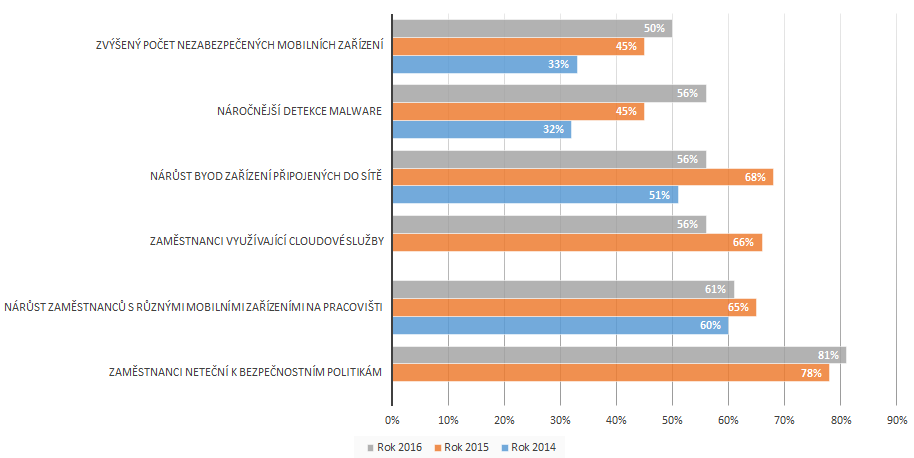
\includegraphics[width=14cm]{img/hrozby}
\caption{Jaké jsou největší hrozby pro bezpečnost koncových zařízení v organizacích účastníků průzkumu? Zdroj: } 
\end{figure}\todo{citovat }

Až 80 procent respondentů si myslí, že mobilní zařízení v jejich firmě byla během posledních dvanácti měsíců cílem útoku malware. Největší hrozbou jsou přenosné počítače a chytré telefony. Velkým rizikem je užívání komerčních cloudových aplikací uživateli a BYOD. Většina odborníků si myslí, že rozpočet pro zajištění IT bezpečnosti není dostatečný. 

\begin{figure}[h!]\label{hrozbyUtoky}
\centering
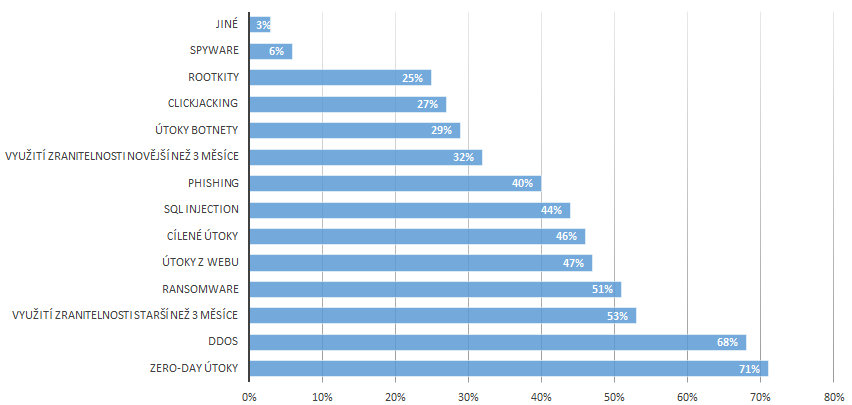
\includegraphics[width=14cm]{img/hrozbyUtoky}
\caption{Jaká část účastníků průzkumu si myslí, že daný typ útoku způsobuje ty nejzávažnější incidenty? Zdroj: } 
\end{figure}\todo{citovat }

Zabezpečení koncových zařízení však hraje v bezpečnostní strategii IT čím dál větší roli. Oraganizace se plánují více soustředit na detekci a reakci, než na prevenci. 





\begin{figure}[h!]\label{hrozbyZarizeni}
\centering
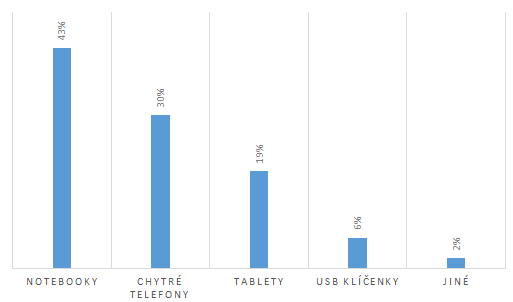
\includegraphics[width=12cm]{img/hrozbyZarizeni}
\caption{Jak velká část účastníků průzkumu si myslí, že největší hrozbou pro organizaci je právě daný typ zařízení? Zdroj: } 
\end{figure}\todo{citovat }



\begin{figure}[h!]\label{hrozbyDuvody}
\centering
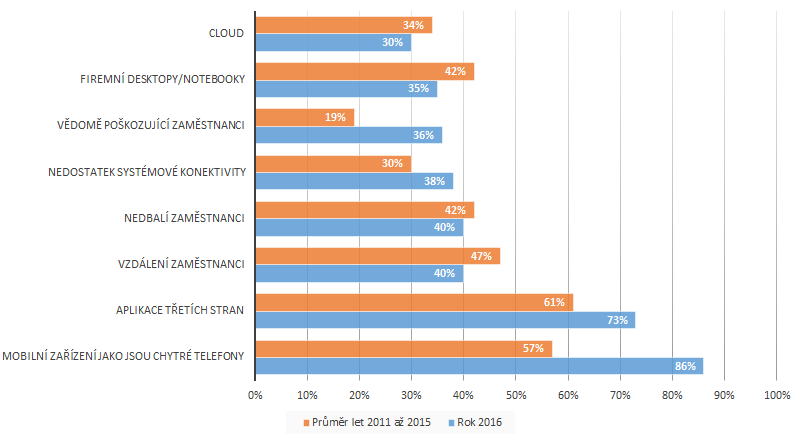
\includegraphics[width=13cm]{img/hrozbyDuvody}
\caption{Jaká část účastníků průzkumu očekává nejvyšší nárůst potencionálního rizika pro bezpečnost IT v daných kategoriích? Zdroj: } 
\end{figure}\todo{citovat }





\section{Specifika bankovního prostředí}
\todo{jak je regulovan banking a ICT v bankingu}

\chapter{Analýza prostředí a požadavků}\label{k2}
 %Ve vybrané bankovní organizaci analyzujte požadavky na připojení vlastních zařízení a identifikujte hlavní hrozby související s nasazením BYOD.
Tato kapitola seznamuje čtenáře s výsledky analýzy vybrané bankovní organizace. Nejdříve je organizace krátce představena a jsou vyjmenována některá specifika tohoto typu organizací. Dále je podrobně analyzován stávající proces připojování nefiremních zařízení do firemní sítě včetně použitých technických prostředků a tento proces je dále podroben analýze souvisejících hrozeb. V neposlední řadě jsou analyzovány známé požadavky na BYOD dané organizaci a typické skupiny uživatelů a jejich potřeb. Závěr kapitoly se zabývá projekty dotýkajícími se problematiky BYOD, které byly v organizaci uskutečněny již dříve.

\section{Popis vybrané organizace}
Zkoumaná organizace je zadavatelem této diplomové práce. Údaje pro tento popis jsou čerpány z výroční zprávy společnosti pro rok 2016. Jedná se o jednu z největších bank v České republice. Byla založena jako státní organizace, nyní se jedná o akciovou společnost. Majoritní podíl akcií drží mateřská společnost ze zahraničí. Typickým akcionářem je fyzická osoba z České republiky.

Čistý zisk v roce 2016 byl více než 13 miliard Kč, celkové provozní výnosy činily více než 31 miliard Kč, provozní náklady 14 miliard Kč.

Banka má více než 7,5 tisíce zaměstnanců, téměř 400 obchodních míst a více než 1,6 milionu klientů.  

Mateřská společnost je jednou z největších evropských finančních skupin. Působí ve více než 70 zemích, má více než 150 tisíc zaměstnanců a obsluhuje více než 32 milionů klientů. 

\section{Vztah autora práce ke zkoumané organizaci}
Autor této práce v době jejího vypracovávání nebyl zaměstnancem zkoumané organizace. Banka, jako zadavatel této práce, interně vedla autora této práce jako externistu, studenta. Analýza probíhala ve spolupráci s oddělením IT Security. Schůzky a konzultace probíhaly napříč odděleními a byly zprostředkovány oddělením IT Security. 

\section{Specifika bankovního prostředí}
Bankovnictví je specifický obor podnikání, a to především z důvodu vysoké státní regulace. Podle své výroční zprávy se Banka musí řídit mimo jiné následujícími právními předpisy:

\textit{
\begin{itemize}
\item zákon č. 21/1992 Sb., o bankách,
\item zákon č. 256/2004 Sb., o podnikání na kapitálovém trhu,
\item zákon č. 90/2012 Sb., o obchodních korporacích,
\item zákon č. 257/2016 Sb., o spotřebitelském úvěru, (účinný od 1. 12. 2016)
\item zákon č. 284/2009 Sb., o platebním styku,
\item zákon č. 38/2004 Sb., o pojišťovacích zprostředkovatelích a samostatných likvidátorech pojistných událostí a o změně živnostenského zákona,
\item zákon č. 253/2008 Sb., o některých opatřeních proti legalizaci výnosů z trestné činnosti a financování terorismu,
\item zákon č. 69/2006 Sb., o provádění mezinárodních sankcí,
\item zákon č. 563/1991 Sb., o účetnictví,
\item zákon č. 101/2000 Sb., o ochraně osobních údajů,
\item zákon č. 143/2001 Sb., o ochraně hospodářské soutěže,
\item zákon č. 136/2011 Sb., o oběhu bankovek a mincí,
\item zákon č. 190/2004 Sb., o dluhopisech,
\item zákon č. 240/2013 Sb., o investičních společnostech a investičních fondech,
\item zákon č. 89/2012 Sb., občanský zákoník,
\item zákon č. 277/2013 Sb., o směnárenské činnosti,
\item zákon č. 634/1992 Sb., o ochraně spotřebitele,
\item nařízení EU č. 596/2014 o zneužívání trhu,
\item nařízení EU č. 575/2013 o obezřetnostních požadavcích na úvěrové instituce a investiční podniky a navazující prováděcí nařízení Evropské komise,
\item nařízení EU č. 648/2012 o OTC derivátech, ústředních protistranách a registrech obchodních údajů (EMIR).
\end{itemize}
}

Banka, jako provozovatel kritické infrastruktury státu, též spadá pod \textbf{zákon č. 181/2014 Sb. o kybernetické bezpečnosti}, což s sebou mimo jiné nese nutnost reportovat kybernetické incidenty.

Vzhledem k vysoko kladeným nárokům na tento typ společností je nezbytně nutné mít jasně nastavené a kontrolované procesy. Podle výroční zprávy společnosti by z hlediska rizik spojených s nesouladem s regulatorními předpisy znamenalo \textit{naplnění některých z rizik  možné důsledky v podobě vedení sporů s regulatorními orgány, institucemi či klienty, riziko finančních pokut, náhrady škod či nákladů na nápravná opatření a dále riziko ztráty reputace a dobrého jména u klientů i široké veřejnosti, a tím další možné finanční ztráty.}

\subsection{Řízení rizik}
Problematika BYOD spadá pod operační rizika. Banka používá pro řízení operačních rizik přístup AMA -- Advanced Measurement Approach. Při zajišťování informační bezpečnosti vychází z norem ISO/IRC 2700x. Pro řízení rizik se používá nástroj RSA GRC -- Archer.

Hodnocení řízení rizik provádí interní audit


\section{Aktuální stav připojování soukromých zařízení}
Podle aktuální praxe ve zkoumané společnosti je připojení zařízení, které není ve vlastnictví společnosti, a to s ohledem na pracovní informační potřeby pracovníků, možné, ovšem toto je hodnoceno jako nesoulad s dobrou praxí a interními předpisy společnosti. Proto musí být pro každý takový případ udělena bezpečnostní výjimka.

\subsection{Proces udělení bezpečnostní výjimky}
Žádosti o připojování nefiremních zařízení se vyřizují pomocí aplikace Service desk. Jedná se o interní aplikaci vyvinutou a spravovanou uvnitř firmy za účelem řízení IT procesů. Proces pro udělení bezpečností výjimky za účelem připojení zařízení, které není ve vlastnictví společnosti, je ilustrován v diagramu \ref{vyjimka}.

\begin{figure}[h!]
\centering
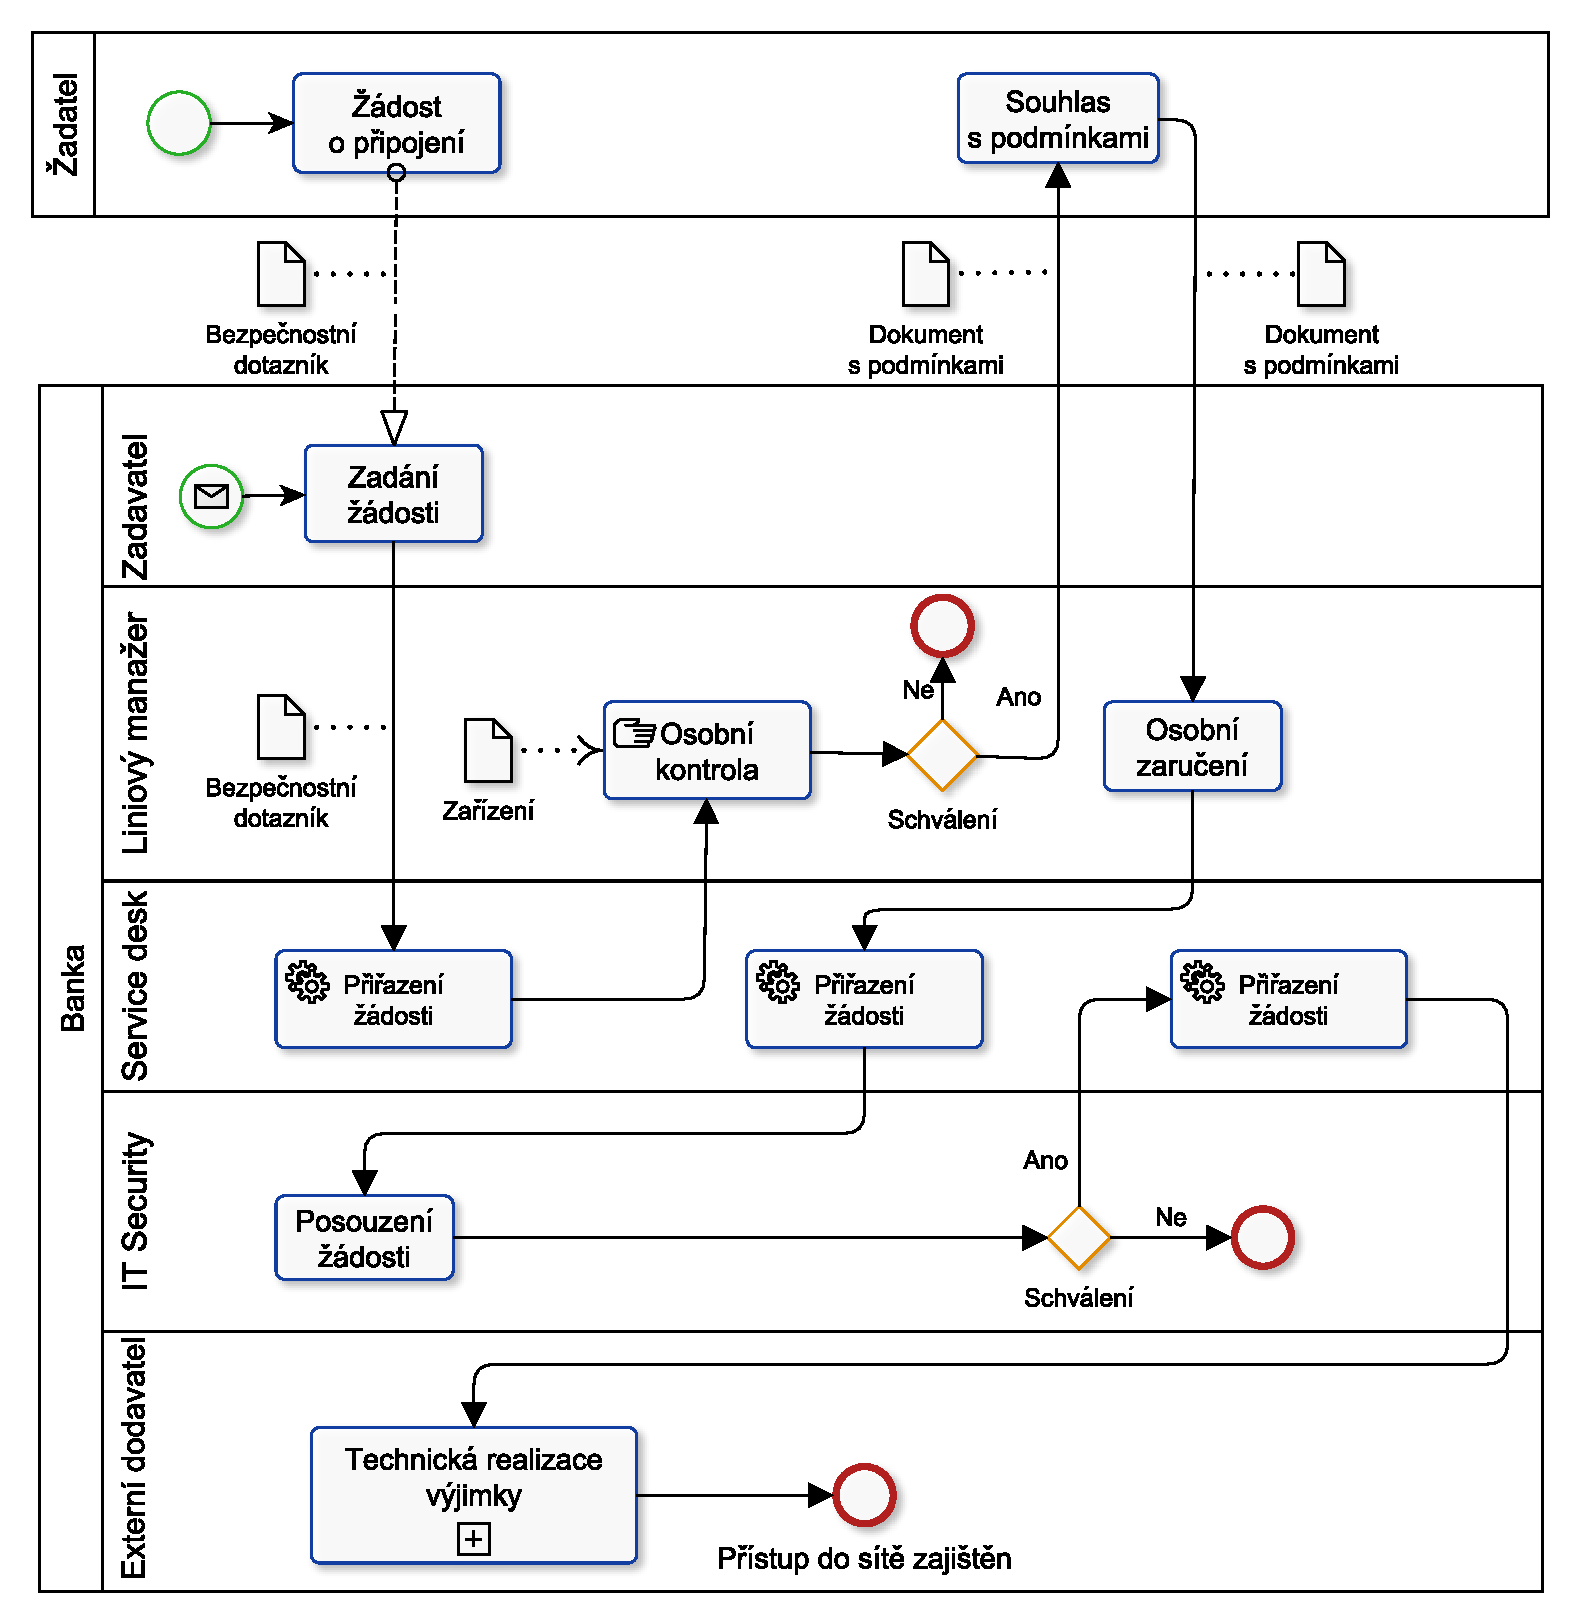
\includegraphics[width=13cm]{img/vyjimkaBPMN}
\caption{Vizualizace procesu pro připojení nefiremního zařízení do vnitřní sítě.\label{vyjimka}} 
\end{figure}

Jelikož žadatel nemá se svým zařízením přístup do vnitřní sítě a tedy ani ke službám aplikace Service desk, je předpokládáno podání žádosti jinou osobou. Jelikož bezpečnostní standardy neumožňují, aby osoba schvalovala vlastní žádost, předkladatelem žádosti nemůže být liniový manažer pod kterého organizačně spadá osoba žadatele. Součástí žádosti je vyplněný bezpečnostní dotazník. 

Dotazník v obecné části obsahuje osobní údaje žadatele, odůvodnění žádosti, typy dat, se kterými bude pracovník nakládat či další informace o vlastnictví zařízení. Technická část dotazuje MAC adresu, použité operační systémy, přítomnost virtualizace, splnění licenčních podmínek software či přítomnost a aktuálnost bezpečnostního software (antivir, firewall, šifrování).

Vytvořený servisní případ žádosti je dále přidělen liniovému manažerovi pod kterého osoba žadatele organizačně spadá. Liniový manažer provede osobní kontrolu zařízení a podepíše se žadatelem dokument specifikující požadavky na žadatele a zařízení. Mezi podmínky patří jednoznačná identifikovatelnost žadatele v rámci informačních systémů společnosti, správnost údajů uvedených v bezpečnostním dotazníku, splnění bezpečnostních politik či splnění licenčních podmínek. Schválením žádosti a jejím postuopením dále se liniový manažer zaručuje za svého podřízeného pracovníka.

Schválenou žádost dále přezkoumá pracovník oddělení IT security. Pokud žádost shledá oprávněnou, předá ji na externí firmu, která udělení bezpečnostní výjimky technicky realizuje. Realizace spočívá ve vytvoření přístupových účtů, přidělení přístupových oprávnění a zadání výjimky pro zařízení do systému spravujícímu přístup do sítě. 

\subsection{Další procesy související s BYOD}
Další procesy jsou buďto triviální, nebo se vymykají rámci této práce a proto nebudou podrobněji analyzovány.

Ve zkoumané organizaci existuje WiFi síť pro hosty.  Je určena především pro návštěvy za účelem obchodních jednání. Přístup k této síti jednoduše vytvoří zaměstnanec Banky ve speciální aplikaci. Pro dlouhodobější vytvoření přístupu zadá zaměstnanec požadavek do systému Service desk.
Připojování nefiremních mobilních zařízení v době psaní této práce nebylo povoleno a tedy neexistoval související proces. Připojování firemních zařízení je mimo rámec této práce. 

\subsection{Připojení z technického hlediska}

Pro správu nefiremních zařízení ve své síti používá zkoumaná společnost nástroj MAB Keeper od společnosti AleFIT. Ta jej v \cite{MABKeeper} definuje následovně: \textit{Aplikace slouží ke správě MAC adres zařízení, která jsou v autentizačním systému použita pro autentizaci, ale nejsou kompatibilní se standardem 802.1x, nebo správě zařízení, u nichž se MAC adresa využívá jako náhradní způsob autentizace. AleFIT MAB Keeper také umožňuje díky několika modulům kontrolovat a časově omezit přístup kontraktorů, konzultantů i BYOD zařízení do firemní sítě, stejně jako využít workflow pro realizaci re-image stanic.} Jedná se o nadstavbu používaného systému Cisco Identity Service Engine (ISE).


Systém ISE řídí nasměrování zařízení do patřičné VLAN na základě adresy MAC. podle příslušnosti k patřičné VLAN má připojené zařízení zajištěna přístupová práva. Ta se řídí pomocí seznamů pro řízení přístupu neboli anglicky Access controll list (ACL). Jedná se tedy o správu připojených zařízení na úrovni topologie sítě. 

Výjimky je možné najít v aplikaci MAB keeper v záložce Approved devices. MAB Keeper tak slouží pro distribuci správy. Mezi používané techniky se řadí MAC address bypass, což znamená obejití standardní autentifikace pomocí protokolu 802.1.X. Jelikož nefiremní zařízení nemají autorizační certifikát, používá se autorizační funkce. Ta zohledňuje MAC adresu a přihlašovací údaje. Uživatelé s vlastními zařízeními a uznanou výjimkou se mohou být přiřazeni do stejné VLAN jako firemní zařízení.


Z hlediska použití bezdrátových sítí WiFi existuje datová síť a síť pro hosty. Pro přístup k datové síti je nutný certifikát, a to především z důvodu fyzické dostupnosti signálu sítě i mimo objekty firemní objekty. Není v plánu další rozšiřování datových WiFi sítí.  

WiFi síť pro hosty je určena pro krátkodobé návštěvníky a umožňuje pouze přístup k síti internet. Důvodem pro její existenci jsou především prezentace obchodních partnerů a další datově méně náročné činnosti. Probíhá na ní URL filtrace.

Jednodenní přístup mohou vytvořit zaměstnanci banky pomocí speciální aplikace. Vytvoření dlouhodobějšího přístupu je možné a vytváří se pomocí žádosti v aplikaci Service desk. 

\section{Cisco ISE}
Společnost Gartner v \cite{GartnerNAC} popisuje Cisco ISE jako jako technologii založenou na protokolu RADIUS. Pokročilé funkce NAC potřebují užitích dalších komponent jako třeba TrustSec Security Group Tag. S použitím device profiling and feed service umožňuje analyzovat provoz a vytvářet reporty o připojených zařízeních.

Balík Cisco AnyConnect sjednocuje další funkce jako jsou VPN, NetFlow nebo ochrana proti škodlivému software. V ISE verze 2.0 je zabudována podpora pro certifikáty, Active Directory či TACACS+.

\section{Analýza aktuálních bezpečnostních rizik spojených s BYOD}
Jelikož metodika analýzy rizik je pro firemního partnera citlivou informací, není pro potřeby této práce možné pracovat s interními metrikami. Vhodné metriky pro hodnocení rizik spojených s kybernetickou bezpečností uvádí zákon o kybernetické bezpečnosti, vyhláška č. 316/2014 Sb., viz \cite{Zakon1}.

Hodnocení rizik používá následující funkci:

$$ riziko = dopad * hrozba * zranitelnost $$


Zákon o kybernetické bezpečnosti udává v § 4, bod (4) vzhledem k bezpečnosti informačních systémů ke zvážení následující hrozby:

\textit{
\begin{enumerate}[label=(\alph*)]
\item porušení bezpečnostní politiky, provedení neoprávněných činností, zneužití oprávnění ze strany uživatelů a administrátorů,
\item poškození nebo selhání technického anebo programového vybavení,
\item zneužití identity fyzické osoby,
\item užívání programového vybavení v rozporu s licenčními podmínkami,
\item kybernetický útok z komunikační sítě,
\item škodlivý kód (například viry, spyware, trojské koně),
\item nedostatky při poskytování služeb informačního systému kritické informační infrastruktury, komunikačního systému kritické informační infrastruktury nebo významného informačního systému,
\item narušení fyzické bezpečnosti,
\item přerušení poskytování služeb elektronických komunikací nebo dodávek elektrické energie,
\item zneužití nebo neoprávněná modifikace údajů,
\item trvale působící hrozby a
\item odcizení nebo poškození aktiva.
\end{enumerate}
}

a dále pak v bodu 6:
\textit{
\begin{enumerate}[label=(\alph*)]
 \item porušení bezpečnostní politiky, provedení neoprávněných činností, zneužití oprávnění ze strany administrátorů kritické informační infrastruktury,
 \item pochybení ze strany zaměstnanců,
 \item zneužití vnitřních prostředků, sabotáž,
 \item dlouhodobé přerušení poskytování služeb elektronických komunikací, dodávky elektrické energie nebo jiných důležitých služeb,
 \item nedostatek zaměstnanců s potřebnou odbornou úrovní,
 \item cílený kybernetický útok pomocí sociálního inženýrství, použití špionážních technik a
 \item zneužití vyměnitelných technických nosičů dat.
\end{enumerate}
}

Zranitelnosti jsou vzhledem k zákonem udávaným typům pro tuto analýzu vzhledem k nastaveným bezpečnostním opatřením pro ochranu informačních systému uvnitř zkoumané společnosti konstantní.

Dále je provedeno hodnocení rizik spojených s připojováním nefiremních zařízení aktuálním postupem pomocí metrik zákona o kybernetické bezpečnosti.

Hrozby e), h), i), j), k) ve vztahu k aktuálně praktikovanému připojování uživatelů s nefiremními zařízeními neexistují, a proto jsou podle stupnice ze \cite{Zakon1} nízké.

Hrozba a) je pravděpodobná, jelikož bezpečnostní politiky není možné vynutit. Hrozbu je tedy nutné hodnotit jako \textbf{střední až vysokou}. Jelikož porušení bezpečnostních politik může mít vliv na chod systémů avšak v omezeném rozsahu a časovém období, lze jej hodnotit jako \textbf{střední}. Výsledné riziko je tedy \textbf{střední až vysoké} a podle použité metodiky by měly být v případě nižší náročnosti zahájeny systematické kroky k jeho odstranění.

Hrozba b) je málo pravděpodobná a její dopad by byl v omezeném období a malého rozsahu. Výsledné riziko je tedy \textbf{nízké}.

Hrozba c) je reálná v případě odcizení zařízení a jeho následném použití pro připojení k firemní síti. Je málo pravděpodobná a nejsou známy žádné případy. Stupeň hrozby je tedy \textbf{střední}. Dopad je v omezeném rozsahu a časovém období, je tedy \textbf{střední}. Riziko je tedy \textbf{střední} a je tolerovatelné pouze pokud by protiopatření byla vyšší náročnosti.

Hrozba d) je pravděpodobná jelikož není možné kontrolovat veškerý nainstalovaný software na zařízení a shodu licenčního ujednání s firemními podmínkami. Stupeň hrozby je tedy \textbf{střední až vysoký}. Jelikož pracovník se smluvně zavázal, že nelicencovaný software používat nebude, břímě odpovědnosti leží na jeho osobě. Případné dopady tedy mohou být přeneseny na něj a hodnocení dopadů je tak \textbf{nízké}. Výsledné riziko je tedy \textbf{nízké až střední}.

Hrozba f) je spíše pravděpodobná. Přestože se uživatel zavázal k používání zazáplatovaného systému a aktuální antivirové ochrany, není možné toto vynutit a monitorovat bezpečné chování uživatele. Tuto hrozbu je možné hodnotit jako \textbf{střední až vysokou}. Teoretický dopad může být nezanedbatelného rozsahu a způsobit škodu. Riziko je tedy \textbf{střední až vysoké} a měly by být zahájeny kroky k jeho odstranění.

Hrozba l) je reálná, stávající opatření nijak neznesnadňují případnému pachateli odcizení aktiv, předpokládaná realizace hrozby však není častá a lze ji proto hodnotit jako \textbf{nízkou až střední}. Finanční ztráty by mohly být znatelné, avšak rozsah dopadu se zdá být omezený, dopad tak lze hodnotit jako \textbf{nízký} a celkové riziko jako \textbf{nízké až střední}.

Vzhledem k dalším uvedeným hrozbám lze konstatovat, že připojování nefiremních zařízení na základě výjimek oproti firemním zařízením znamená zvýšení pravděpodobnosti hrozby c), f) a g), a proto je třeba jim věnovat pozornost. 

\subsection{Zhodnocení analýzy rizik}\label{analyzaRizik}
Při porovnání s užitím firemního zařízení byla při stávajícím způsobu připojování nefiremního zařízení identifikována zvýšená pravděpodobnost realizace některých hrozeb potažmo rizik. Tato práce si klade za cíl hodnotit možná řešení především z hlediska bezpečnosti a navrhnout tak řešení, která identifikovaná rizika zásadním způsobem sníží.

\subsection{Analýza hrozeb souvisejících s nasazením BYOD}
Jelikož BYOD zařízení již nyní ve firemní síti existují, nasazení navrhovaného BYOD programu nijak nezvyšuje pravděpodobnost žádné ze známých hrozeb. V této práci navrhované řešení se soustředí na bezpečnost a tedy nejenom že nezvyšuje pravděpodobnost realizace známých bezpečnostních hrozeb oproti stávajícím firemním zařízením, ale naopak zvyšuje bezpečnost oproti aktuálnímu způsobu připojování nefiremních zařízení.


\section{Analýza požadavků na připojení vlastních zařízení} 
Formou konzultací se zaměstnanci zkoumané společnosti napříč různými odděleními bylo identifikováno několik požadavků a potřeb.

\subsection{Obecné požadavky}\label{obecnePozadavky}

Jedním z hlavních požadavků je přiměřenost z hlediska nákladů. Návrh řešení je třeba obhájit před vedením společnosti, které schvaluje rozpočty projektů. Zároveň je žádoucí, aby řešení mělo kladné přijetí od potencionálních uživatelů, tak aby byli ochotni jej využívat a náklady na zavedení nebyly vynaloženy zbytečně.  

Smyslem vytvoření BYOD programu je vytvoření uceleného návrhu, který umožní zaměstnancům v odůvodněných případech využívat vlastní zařízení a především zvýší bezpečnost existujících BYOD, které se nyní objevují převážně u kontraktorů. Existující riziko, plynoucí z nespravovaných nefiremních zařízení v síti, je třeba potlačit, což je nejsilnějším argumentem pro prosazení projektu.

Důvody k zavedenní řešení BYOD lze tedy rozdělit na technologicko-sociální a obchodní. Je zřejmé, že vzhledem k nastoleným trendům je nutné nastolit firemní strategii pro BYOD. Pokud by se řešení nenašlo, nefiremní zařízení se přesto budou rozšiřovat, ovšem nebudou pod kontrolou firemního IT oddělení. To v důsledku znamená, že nebude možné kontrolovat rizika ani náklady s tímto spojené. 

Z pohledu oddělení IT Security je majoritním důvodem pro řešení otázky BYOD aktuální stav, kdy jsou nefiremní zařízení připojována na základě bezpečnostních výjimek. Tento stav je nežádoucí a je identifikován jasný požadavek pro nastolení rámce, který eliminuje hrozby z toho plynoucí.


\subsection{Identifikované potřeby}\label{identifikovanePotreby}
\begin{itemize}
    \item Tablety pro vrcholový management
    \item Vlastní notebooky
    \item Vlastní počítače Apple
    \item Firemní notebooky externích konzultantů
    \item Přístup k dokumentům ze soukromých tabletů
    \item Přístup k emailu či kalendáři z osobního chytrého telefonu
\end{itemize}

\subsection{Identifikované služby}\label{identifikovaneSluyby}
Z hlediska souvisejících služeb poskytovaných IT byly identifikovány služby typu \textbf{PIM}\footnote{Personal Information Management} neboli služby pro správu osobních informací, typicky se jedná o kalendář, email a další komunikační a organizační systémy, jimiž jsou například Oultook a Skype for Bussiness. Dále je třeba zprostředkovat služby pro \textbf{tvorbu a sdílení dokumentů}. Typicky se jedná o Microsoft Office či Atlassian Confluence. V neposlední řadě je nutný přístup k \textbf{business aplikacím}.

\subsection{Identifikované typy zařízení}
Co se týče různých typů zařízení, je třeba do BYOD programu zařadit firemní chytré telefony včetně zařízení BlackBerry a tablety. Co se týče nefiremních či osobních zařízení je třeba zohlednit chytré telefony, tablety, notebooky či notebooky od firmy Apple.

\subsection{Identifikovaní uživatelé}
Jako uživatelé byli identifikováni zaměstnanci Banky, externí dodavatelé, kontraktoři a klienti.

Skupinou uživatelů, která z principu přichází s vlastními zařízeními jsou externisté, jež Banka z pravidla najímá pro účely projektů. Tito uživatelé můžou pracovat na živnostenský list, nebo mohou být zaměstnanci externího dodavatele. Uživatelé pracující na živnostenský list používají zpravidla soukromá zařízení, zaměstnanci externích dodavatelů používají zpravidla zařízení ve vlastnictví a správě svého zaměstnavatele.

Jako nejčastější typy pracovníků z externích zdrojů byli identifikováni:
\begin{itemize}
    \item Projektoví manažeři
    \item Vývojáři
    \item IT konzultanti
\end{itemize}

Projektoví manažeři jsou zpravidla najímáni pro své know-how z jiných projektů. Mezi priority v jejich potřebách patří firemní služby typu PIM (kalendář, email,\ldots) nástroje pro vytváření dokumentů a kolaboraci, přístup k dokumentům a datům či další nástroje potřebné k řízení projektů. 

IT konzultanti potřebují používat nástroje, dokumenty a služby spojené s danou konzultační činností, kterou Bance poskytují. Problematika vývojářů je popsána v odstavci \ref{potreby_vyvojar}.

V případě externích pracovníků je obzvláště nutné dbát na ochranu firemních dat. Je užitečné mít možnost zajistit, že po ukončení své činnosti tito pracovníci dále nebudou moci nakládat s firemními aktivy. Tito pracovníci se musí řídit vnitřními směrnicemi banky. V případě bezpečnostního incidentu je možné tyto pracovníky nebo jejich zaměstnavatele právně postihovat, typicky pokutou, a to na základě standardně uzavíraného právního vztahu.

Zájem o používání vlastních zařízení však mají i zaměstnanci Banky. Identifikováni byli především uživatelé z vedení společnosti (počítače Mac, tablety iPad) a vývojáři. Pokud se vinou svého vlastního zařízení dopustí bezpečnostního incidentu zaměstnanec banky, je jeho zodpovědnost obtížněji vymahatelná.

\subsection{Způsoby připojení k síti}
Z hlediska připojení k síti byly identifikovány následující možnosti: připojení do sítě LAN, připojení do lokální WiFi a připojení skrze síť internet a mobilní připojení.

\subsection{Způsob podpory od IT oddělení}
Momentálně IT oddělení poskytuje end-to-end podporu. To znamená, že dodaní služeb je podporováno kompletně od zdroje, přes dodání po podporu koncových zařízení. Tento model není trvale udržitelný pro BYOD, kdy není možné podporovat všechna koncová zařízení a je tedy třeba zavést i model, kde je podporována pouze samotná služba. Návrh způsobu podpory pro BYOD je rozveden v kapitole \ref{dalsi_opatreni}.

\subsection{Identifikace potřeb specifického uživatele -- vývojáře}\label{potreby_vyvojar}
Vývojáři patří mezi prioritní skupinu uživatelů, pro které je třeba připravit projekt BYOD. Právě mezi vývojáři je velké množství kontraktorů, kteří si přinášejí své vlastní nefiremní zařízení. Vývojáři však mají vyšší požadavky než běžní uživatelé. Konzultací se zástupci vývojářů v Komerční bance byly identifikovány následující potřeby. 

Vývojář potřebuje mít na zařízení, na kterém vyvíjí, administrátorská oprávnění. Je to především z důvodu instalace pomocných nástrojů, tak z důvodu přístupu k některým systémovým funkcím operačního systému, například pro potřeby testování. Dále má vývojář zvýšené nároky na výpočetní výkon stroje, na kterém němž pracuje, především z důvodu potřeby lokální kompilace zdrojových kódů. 

Vývojáři mají specifické požadavky na nainstalované aplikace. Každý potřebuje vývojové prostředí (Banka nemá sjednoceno, a tedy vývojáři mohou volit nástroj dle svého uvážení, například IntelliJ Idea). Poté jsou to nástroje pro vývoj databází, například Oracle SQL Developer. Dále je nutné přistupovat k dalším databázím. V prostředí zkoumané organizace se používají různé databáze (Oracle, MySQL, MS SQL). Mezi dalšími nezbytnými nástroji byl uveden SSH klient Putty.

Byla zmíněna potřeba přístupu k následujícím službám:
\begin{itemize}
    \item Přihlašování do domény
    \item Přístup k logům -- k centrálnímu systému logů na systému Logman
    \item Přístup k nástroji pro zpracování výstupních streamů Apache Kafka
    \item Přístup k verzovacímu systém GIT na platformě BitBucket
    \item Přístup k systému pro evidenci chyb Atlassian JIRA
    \item Přístup k nástroji pro dokumentaci Atlassian Confluence
    \item Přístup k nástroji pro automatizaci správy software Jenkins
    \item Přístup k testovacím prostředím
    \item Přístup k emailům 
    \item Přístup ke službě Skype for business
    \item Přístup k adresářové službě LDAP
    \item Přístup ke správě identit ITIM
\end{itemize}

Pokud se vývojář připojuje vzdáleně, klade důraz na přístup k verzovacíu systému GIT, přístup k testovacímu prostředí a přístup k logům.

\section{Aktuální stav podpory různých typů zařízení dle typu vlastnictví}


Nejvyšší prioritou je umožnit uživatelům se soukromými zařízeními plný a kontrolovaný přístup ke službám lokální sítě. Není nutné zajišťovat vzdálený přístup pro nefiremní zařízení, je však třeba podporovat vzdálený přístup k emailu. Pro mobilní telefony je třeba zajistit přístup k emailu. Přístup k dokumentům a aplikacím zatím není vyžadován. Byl identifikován požadavek na firemní tablety od vrcholového managementu. Pro ty je třeba zajistit maximální přístup. Uživatelé soukromých tabletů požadují přístup k emailu a dokumentům.

% Please add the following required packages to your document preamble:
% \usepackage{multirow}
\begin{table}[]

\centering

\resizebox{\textwidth}{!}{\begin{tabular}{c|l|l|l|l}
 &  & firemní zařízení & Soukromé zařízení & Zařízení kontraktora \\ \hline
\multirow{2}{*}{Notebook} & Lokálně & Dostupné & Nepodporované ale používané & \multicolumn{1}{l}{Nepodporované ale používané} \\ %\cline{2-5} 
 & Vzdáleně & Dostupné přes VPN & Nepodporované & \multicolumn{1}{l}{Nepodporované} \\ \hline
\multirow{2}{*}{Tablet} & Lokálně & Nedostupné & Nedostupné & \multicolumn{1}{l}{Nedostupné} \\ %\cline{2-5} 
 & Vzdáleně & Nedostupné & Nedostupné & \multicolumn{1}{l}{Nedostupné} \\ \hline
Chytrý telefon & Vzdáleně & Dostupné pro BlackBerry & Nedostupné & \multicolumn{1}{l}{Nedostupné} \\ %\cline{1-1}
\end{tabular}}

\caption{Tabulka aktuálního stavu podpory pro jednotlivé typy zařízení podle typu vlastnictví}
\label{tabulka1}

\end{table}
%\todo{tabulka}


\section{Předešlé projekty}
Projekt na vyhodnocení konceptu BYOD byl v bance započat již v roce 2013. Měl za cíl vyhodnotit rámec pro konkrétní potřeby, scénáře a služby, dále měly být nastaveny předpokládané výstupy a definováno možné řešení. Již v roce 2013 byl citelný příklon uživatelů ke konzumerizaci informačních technologií a prorůstání jiných než-li PC zařízení do firemního prostředí.

V té době se mobilní připojení stalo standardem i pro běžné uživatele a ti tak byli neustále připojeni se svými osobními zařízeními k internetu. Dále byla citelná osobní potřeba zaměstnanců používat svá osobní zařízení i během pracovní doby.

Projekt nastolil možnost zpřístupnění přístupu k emailu i z nefiremních zařízení. Důvodem je zvýšení pracovní efektivity při minimálních dodatečných výdajích. Na mnohých pracovních pozicích by též zavedení BYOD programu umožňovalo flexibilnější pracovní styl. S tím souvisí i snadnější přístup ke klientům. 
Flexibilnější přístup umožňuje lépe uplatňovat techniky křížného prodeje\footnote{Křížný prodej, někdy též křížový prodej (anglicky cross-selling), je obchodní taktika navyšování prodeje, jejímž cílem je prodat více, doporučením souvisejícího zboží nebo služeb, viz \cite{ManagementMania}}. Bezprostřední přístup k informacím by znamenal rychlejší reakci obchodníků a konkurenční výhodu. 

\subsection{Dříve zvažované možnosti pro email}
V minulosti bylo zvažováno několik možností, jak zpřístupnit email a dokumenty na soukromých chytrých telefonech a tabletech.

Exchange ActiveSync snižuje riziko krádeže díky vynucení zadání PIN kódu a možnosti vzdáleného smazání. V jeho prospěch hrála relativně snadná a rychlá implementace. Řešení bylo zamítnuto, protože nenabízelo zašifrování dat. To může znamenat ohrožení dat například při jail-breaku u zařízení iPhone.

V rámci mateřské skupiny se používá řešení Good mail (nyní BlackBerry Work). Toto řešení nevyhovovalo požadavkům vzhledem k vysokým nákladům na implementaci a provoz. Nicméně projekt pro toto řešení stále existuje.

Microsoft Outlook Web App umožňuje prohlížení příloh přímo na serveru a není tedy nutné lokální šifrování dat. Řešení je vhodné jak pro mobilní zařízení, tak tablety a nepřináší žádné dodatečné náklady, jelikož je již implementováno. Uživatelé však nehodnotí uživatelskou přívětivost tohoto řešení příliš kladně.

\subsection{Projekt VDI pro vývojáře a testery}\label{projektVDI}

V Bance též existoval projekt, který se snažil ověřit možnost využití virtuálních strojů pro vývojáře a testery. Důvodem byla snaha získat řešení pro vlastní zařízení kontraktorů, která znamenají bezpečnostní riziko. Dále si Banka od projektu slibovala nalezení řešení problému s využíváním několika zařízení vývojáři, ať už z důvodu vzdálené podpory nebo zvláštních požadavků na výkon.

Test VDI se odehrál v roce 2011, probíhal tři týdny a zúčastnilo se ho 5 vývojářů. Uživatelé po dobu testu prováděli veškeré své pracovní úkony ve virtuálním prostředí. Virtuální stroje běžely na serveru Proliant DL380 G5 s parametry: 4x (2CPUx2jádra) CPU 3000MHz, 24GB RAM a 1,3TB místa na disku. Parametry pro jednotlivé virtuální stroje byly ekvivalentí k PC dvoujádrovým procesorem a 2-4 GB RAM.

Účastníci testu ohodnotili uživatelský zážitek jako dostatečný pro běžné použití. Zaznamenali však nižší odezvu a občasné záseky. Byly identifikovány problémy s periferními zařízeními, například nefungovala čtečka na čipové karty. Odezva vývojářských nástrojů byla odhadem dvakrát pomalejší. Uživatelé hodnotili přechod k virtuálním strojům jako zhoršení uživatelského komfortu oproti fyzickým firemním PC. 

Test prokázal vysoké nároky na diskové úložiště především co se týče počtu požadavků na vstupně/výstupní operace. To znamená nutnost vysoké investice do kvalitního diskového úložiště. Zároveň je nutné zajistit kvalitní konektivitu. Proto bylo rozhodnuto, že VDI není vhodné pro interní vývojáře, protože zvyšuje náklady a nepřináší benefity.

Zároveň test doporučil ke zvážení zkoušený model VDI pro kontraktory, a to pod podmínkou užití vlastního zařízení bez dalších nákladů pro Banku, bez zajištění vysoké dostupnosti a omezení velikosti diskové kapacity pro virtuální stroje na odhadovaných 70-80GB.
 
\chapter{Možné varianty řešení}\label{k3}
 %Analyzujte dostupná existující řešení BYOD, zejména z pohledu bezpečnosti.

Podle společnosti Gartner \todo{citace http://www.gartner.com/it-glossary/bring-your-own-device-byod/} je Bring your own device (BYOD) alternativní strategií pro povolení zaměstnancům, obchodním partnerům a dalším uživatelům používání osobně zvolených a pořízených koncových zařízení pro spouštění podnikových aplikací a přístup k datům.  Běžně zahrnuje chytré telefony a tablety, ale může být použita také pro osobní počítače. Může zahrnovat také dotaci od zaměstnavatele na pořízení zařízení.


Na problematiku nefiremních zařízení je možné nahlížet z různých pohledů. V této kapitole budou představeny různé možnosti dělení zařízení dle různých kategorií a taktéž budou představeny odpovídající řešení.

\todo{vice obecnych kecu o BYOD}

 \section{Různé pohledy na BYOD}
 \subsection{Rozdělení zařízení podle vlastnictví}
 Na základě vlastnictví zařízení je určena míra kontroly firmy zařízeními ve svojí síti.
 
 \subsubsection{Firemní zařízení}
 Jedná se o zařízení, které nakupuje a zároveň spravuje firma. Je ve vlastnictví firmy a pod dohledem IT oddělení. Zařízení plně splňuje politiky firmy a je plně kontrolované.
 
 \subsubsection{Externí firemní}
 Jedná se o firemní zařízení pracovníka externí firmy, jedná se tedy o firemní zařízení, ale o firemní zařízení jiné firmy. Je tedy pod správou IT oddělení externí firmy.
 
 Zařízení splňuje bezpečnostní politiky externí firmy a je kontrolované externí firmou. Není možné zařízení kontrolovat, je však možné vynutit potřebné bezpečnostní politiky smluvním vztahem s externí firmou.
 
 \subsubsection{Externí soukromé}
 Zařízení externího pracovníka, které není kontrolované firemní politikou externí firmy. Není možné jej kontrolovat a je obtížné vynucovat bezpečnostní politiky.
 
 \subsubsection{Zaměstnanec se soukromým zařízením}
 Vlastní zařízení zaměstnanců. Není kontrolované a může představovat bezpečnostní riziko.
 
 \subsection{Rozdělení podle typu zařízení}
 \subsubsection{PC}\todo{zdroj http://www.intel.com/content/www/us/en/tech-tips-and-tricks/pc-vs-mac-the-big-debate.html}
 V užším slova smyslu se jedná o osobní počítače s operačním systémem Windows od firmy Microsoft. Windows je aktuálně nejrozšířenější operační systém pro korporátní zařízení. Systém je určený pro zařízení postavené na architektuře x86. Typicky se jedná o stolní počítače a notebooky. Podle statistiky StatCounter\todo{zdroj: http://gs.statcounter.com/os-market-share/mobile-tablet/czech-republic/} měl operační systém Windows v únoru 2017 90 procentní podíl na trhu operačních systémů pro desktopy podle počtu přístupů na web. Podle celosvětových statistik přístupů na web v souhrnu všech typů zařízení podle StatCounter má však Windows pouze 38,6 procenta přístupů a je zřejmý trend mezi běžnými uživateli v upřednostňování jiných zařízení na úkor PC.\todo{zdroj: http://tech.ihned.cz/internet/c1-65653000-android-predbehne-windows-jako-nejpouzivanejsi-system-na-webu-v-cesku-mu-brani-draha-data}  
 
\begin{figure}[h]
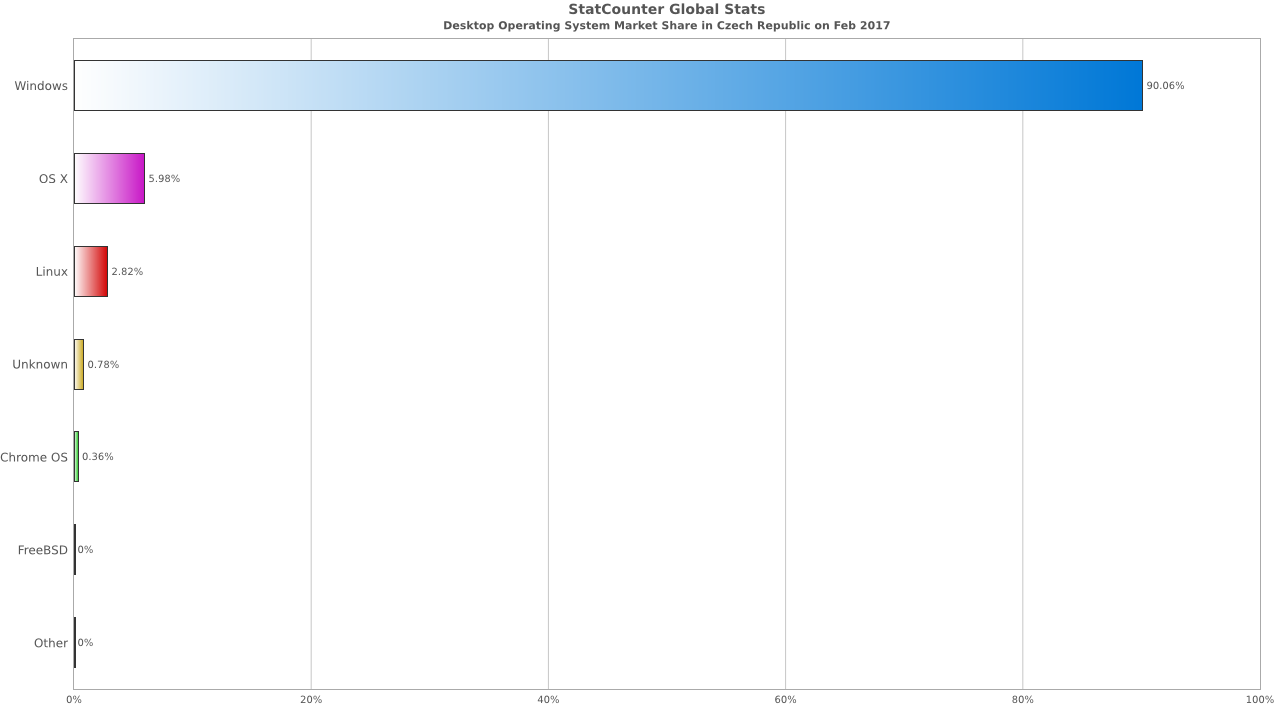
\includegraphics[width=13cm]{img/StatCounter_Desktop}
\caption{Statistika podílu operačních systémů pro desktopy v České republice podle přístupů na web. Převzato z \cite{http://gs.statcounter.com/os-market-share/mobile-tablet/czech-republic/}} 
\centering
\end{figure}\todo{citace}
 
 
 
 \subsubsection{Mac}\todo{zdroj http://www.apple.com/macos/what-is/}
 Počítač s operačním systémem MAC OS. Jedná se o proprietární operační systém pro počítače firmy Apple. Podle StatCounter je jeho podíl na trhu mezi desktopovými operačními systémy podle počtu přístupů na web v České republice necelých šest procent. Populární je zejména ve Spojených státech, kde se jeho podíl mezi desktopovými operačními systémy podle metodiky StatCounteru pohybuje okolo dvaceti procent.
 
 \begin{figure}[h]
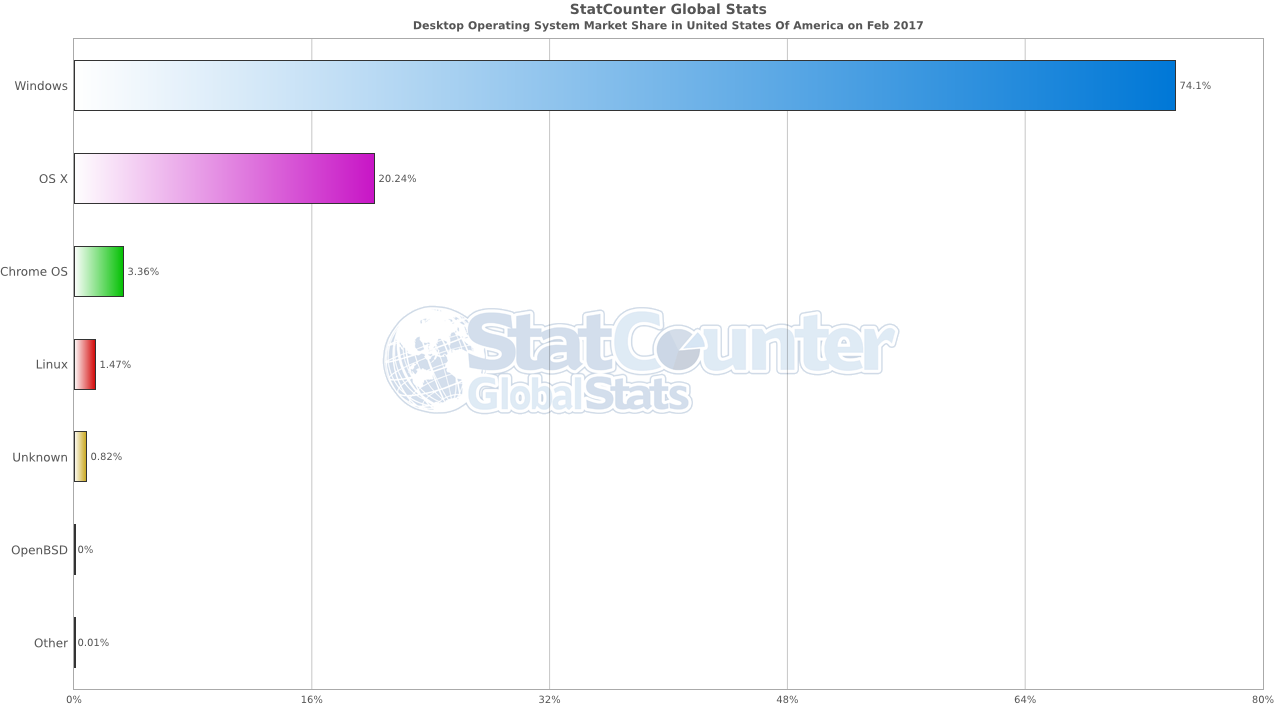
\includegraphics[width=13cm]{img/StatCounter_Destop_USA}
\caption{Statistika podílu operačních systémů pro desktopy v USA podle přístupů na web. Převzato z \cite{http://gs.statcounter.com/os-market-share/mobile-tablet/czech-republic/}} 
\centering
\end{figure}\todo{citace}
 
 
 \subsubsection{Chytrý telefon či tablet}
 Podle společnosti Gartner \todo{citace http://www.gartner.com/it-glossary/smartphone/} je chytrý telefon definován jako mobilní komunikační zařízení používající identifikovatelný otevřený operační systém. Tento systém je podporován aplikacemi třetích stran od komunity vývojářů. Aplikace třetích stran mohou být instalovány nebo odstraněny a mohou být vytvořeny přímo pro operační systém zařízení a aplikační programové rozhraní, případně pro oddělenou vrstvu jakou může být například Java. Operační systém musí podporovat multitaskingové prostředí a uživatelské rozhraní, které dokáže obsloužit více aplikací najednou. Například zobrazení emailu během přehrávání hudby.
 
 Obecněji se jedná mobilní zařízení s možností instalace aplikací. V současné době jsou nejpopulárnější zařízení s operačním systémem Android od firmy Google a iOS od firmy Apple. V České republice je podle metodiky měření společnosti StatCounter pro únor 2017 nejpopulárnější operační systém Android s podílem 68 procent. Operační systém iOS je na drůhém místě s podílem 26 procent. Více než jednoprocentní podíl má již pouze Windows s necelými čtyřmi procenty. \todo{citace http://tech.ihned.cz/internet/c1-65653000-android-predbehne-windows-jako-nejpouzivanejsi-system-na-webu-v-cesku-mu-brani-draha-data a statcounter}
 
 \begin{figure}[h]
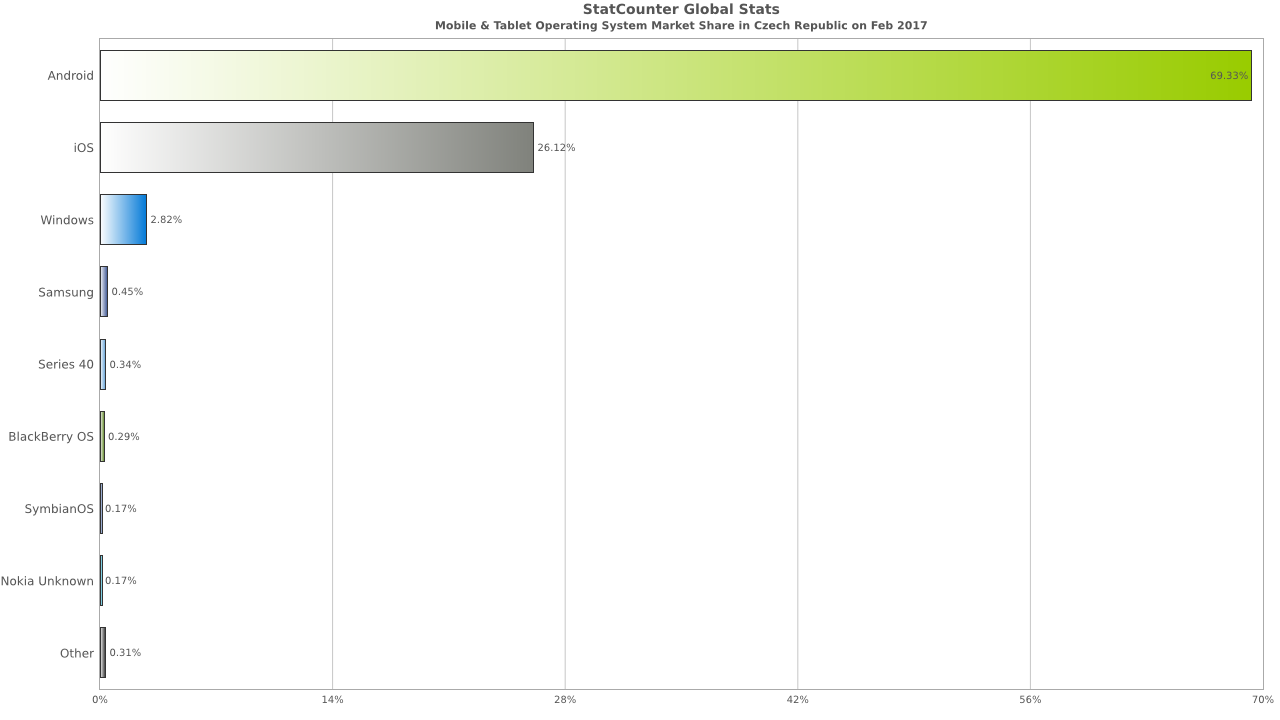
\includegraphics[width=13cm]{img/StatCounter_MobileBar}
\caption{Statistika podílu operačních systémů pro desktopy v České republice podle přístupů na web. Převzato z \cite{http://gs.statcounter.com/os-market-share/mobile-tablet/czech-republic/}} 
\centering
\end{figure}\todo{citace}
 
Celosvětově je zřejmá rostoucí obliba mobilních zařízení mezi uživateli a to především na úkor klasických PC s operačním systémem Windows. Vzhledem k postupné změně návyků uživatelů je třeba, aby firemní prostředí na tento trend vhodně reagovalo. 


\begin{figure}[h]
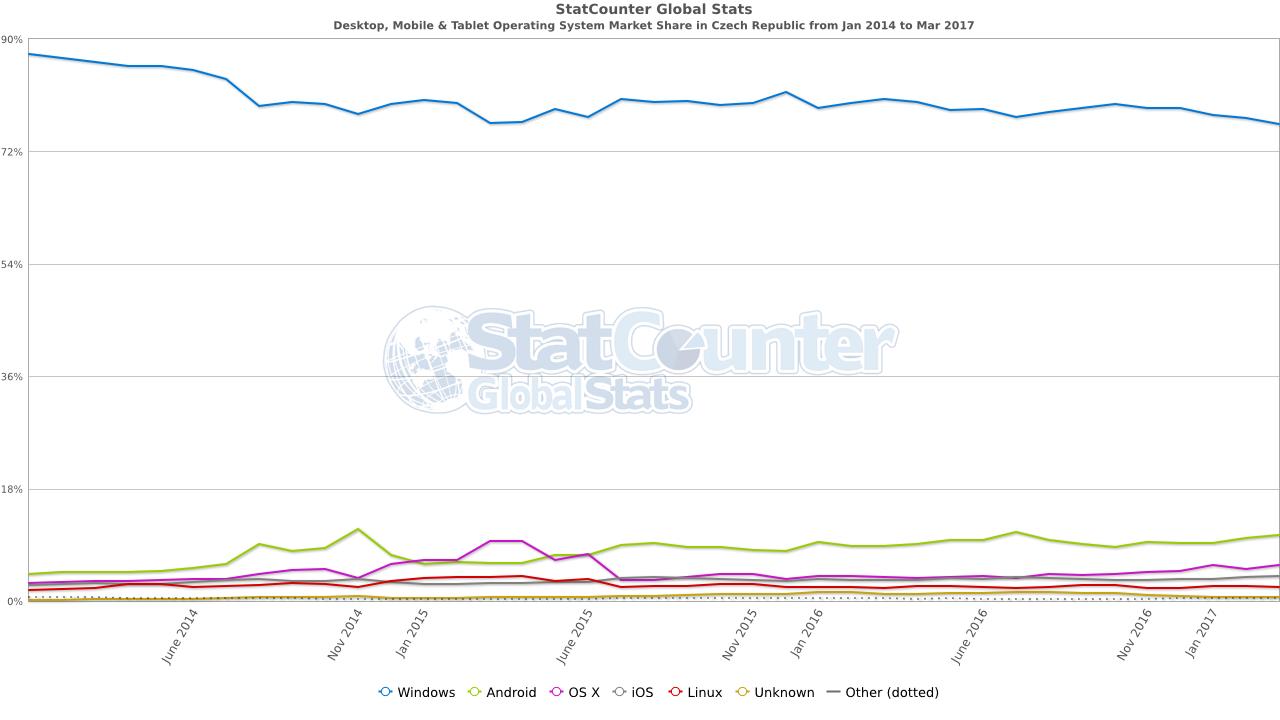
\includegraphics[width=13cm]{img/StatCounter_VyvojVse}
\caption{Statistika podílu všech operačních systémů pro desktopy v České republice podle přístupů na web. Převzato z \cite{http://gs.statcounter.com/os-market-share/mobile-tablet/czech-republic/}} 
\centering
\end{figure}\todo{citace}

\begin{figure}[h]
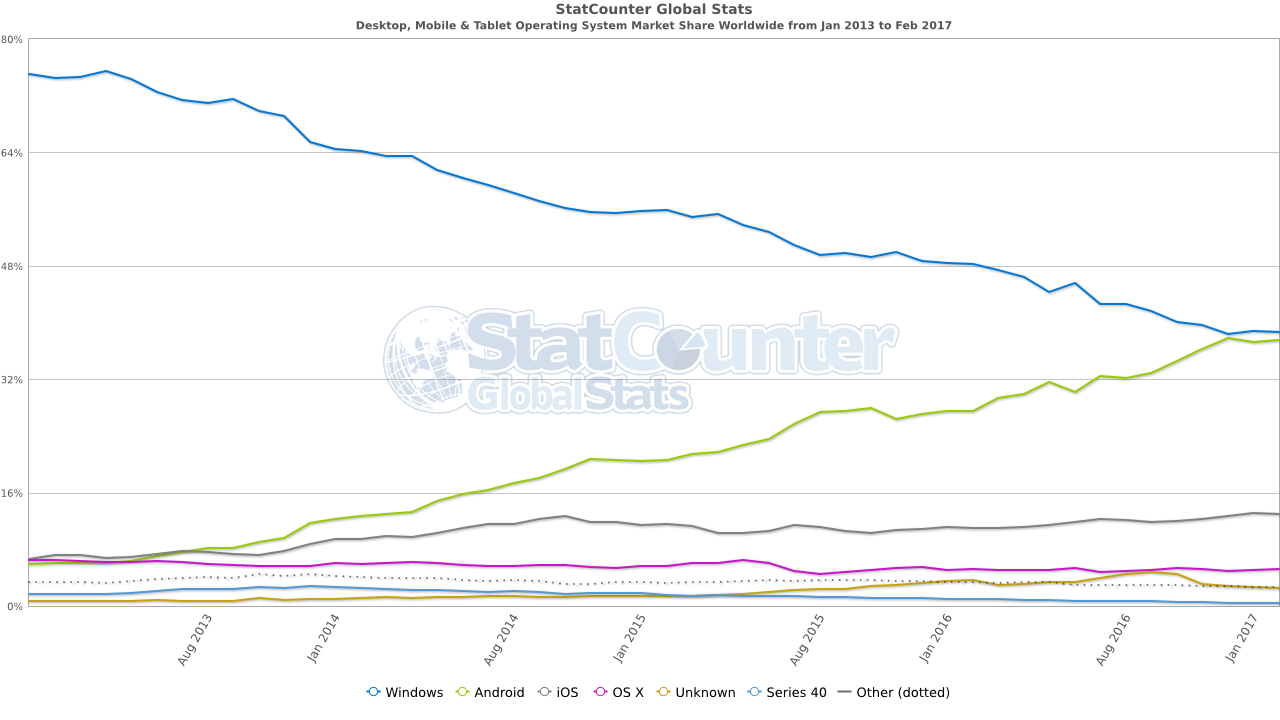
\includegraphics[width=13cm]{img/StatCounter_All_Worldwide}
\caption{Statistika podílu všech operačních systémů celosvětově podle přístupů na web. Převzato z \cite{http://gs.statcounter.com/os-market-share/}} 
\centering
\end{figure}\todo{citace}
 
Od těchto zařízení se nepředpokládá nutnost přístupu k podnikovým aplikacím, ale je vyžadován okamžitý přístup k emailům, kontaktům či dokumentům a to nezávisle na místě použití.
 
 
 %%%%%%%%%%%%%%%%%%%%%%%%%%%%%%%%%%%%%%%%%%%%%%%%%%%%%%%%%%%%%%%%%%%%%%%%%%%%%%%%%%%%%%%%%%%%%%%%%%%%%%%%%%%%%%%%%%%%%%%%%%%%%%%%%%%
 \subsection{Rozdělení podle typu přístupu do datové sítě}
 \subsubsection{Ethernet}\todo{citace http://www.pcmag.com/encyclopedia/term/42781/ethernet}
 Jedná se o pevné připojení do korporátní sítě pomocí kabelu. Je vhodné pro firemní počítače, není vhodné pro zařízení typu mobilní telefon či tablet.
 
 Je definované ve standardu IEEE 802.3 \todo{Naflakat sem vic nesmyslu ze standardu}
 
 \subsubsection{Wi-Fi} \todo{http://www.pcmag.com/encyclopedia/term/54444/wi-fi}
 
 Bezdrátové připojení pomocí Wi-Fi sítí. Jedná se o standardní technologii pro bezdrátové sítě WLAN. Tento typ připojení je vhodný jak pro přenosné počítače, tak pro mobilní telefony či tablety.
 
 Wi-Fi je definovaná standardem IEEE 802.11
 
 \subsubsection{VPN} \todo{citace http://www.cisco.com/c/en/us/about/press/internet-protocol-journal/back-issues/table-contents-18/what-is-a-vpn.html}
 Virtual private network, čili vzdálené připojení do firemní sítě. Hlavním smyslem VPN je vytvořit soukromou síť pomocí tunelování a nebo šifrování skrze veřejný internet tak, aby uživatelé mohli vzdáleně přistupovat ke službám dostupným pouze zevnitř sítě.
 
 
 %%%%%%%%%%%%%%%%%%%%%%%%%%%%%%%%%%%%%%%%%%%%%%%%%%%%%%%%%%%%%%%%%%%%
 
 
 
 \section{Známé způsoby řešení BYOD}\todo{Zejmena z pohledu bezpecnosti}

\todo{doplnit typy hypervizoru/ typy virtualizace}
 
 \subsection{Centralizovaná virtualizace}
 Microsoft remote desktop, VMWare Horizon, Citrix XenDesktop
 \missingfigure{Magic quarter pro virtual dektopy}
 
 \todo{doplnit povidacky}
 
 \subsection{Distribuovaná virtualizace}
 Oracle Virtualbox, VMWare Fusion, VMWare Workstation, VMWare Fusion, VMWare Player, VMWare Horizon Flex
 
 \missingfigure{Taky nejaky hezky grafek}
 
 \subsection{DaaS}
 \todo{pouzit a citovat http://www.tomsitpro.com/articles/desktop-as-a-service-providers,2-838.html}
 Desktop as a service
 VMWare Horizon Air, Citrix XenDesktop, Amazon Work Spaces
 
 \todo{doplnit povidacky}
 
 \subsection{Rozlišení na úrovni sítě}
 Cisco ISE plus a jiné. \todo{Dostudovat a doplnit síťové BYOD}
 
 
 \subsubsection{Virtualizace aplikaci}
 Další možností je nevirtualizovat celý operační systém, ale pouze aplikace. Mezi výhody patří snadná aktualizace aplikací, snadná správa přístupu k aplikacím či nenáročnost na výpočetní výkon klienta.
 
 Mezi hlavní nevýhody patří problémy s periferiemi jako např. tiskárny či nutnost stálé a kvalitní konektivity.
 
  Nejznámějšími poskytovateli virtualizace aplikací jsou Citrix XenApp, Citrix XenDesktop, VMware Horizon, Dell vWorkspace, and Microsoft RDSH\todo{překlad}
 
 
 \subsubsection{EMM/EMS}
 Enterprise mobility management nebo též Enterprise Mobility suite umožňují integrovat a spravovat mobilní zařízení v rámci firemní infrastruktury.
 Dle agentury Gartner jsou EMM balíky lepidlem, které připojuje mobilní zařízení do firemní infrastruktury. \cite{Gartner_EMM_2016}
 
 EMM mají následující funkce:
 \begin{itemize}
     \item nastavují zařízení a aplikace pro nasazení ve firemním prostředí
     \item sledují dodržení firemních politik a spravují firemní aktiva
     \item snižují riziko ztráty dat, krádeže či dalších incidentů řízením šifrování dat, přístupových práv, sdílených zařízení, obalování aplikací či zamknutí zařízení.
     \item umožňují vzdálenou podporu zařízení pro IT oddělení
 \end{itemize}
 

 
 
 
  \subsection{MDM}
 Mobile device management je software pro správu mobilního zařízení. Je podmnožinou EMM. Mezi základní funkce tohoto software patří podle \todo{citace: FEL BYOD vosykto} patří:
 \begin{itemize}
     \item Automatické nastavení mobilního zařízení. Umožňuje IT oddělení nastavit zařízení podle firemních potřeb. To zahrnuje instalaci bezpečnostních certifikátů, nastavení uživatelských účtů či dalších nastavení umožňující přístup k firemní síti.
     \item Možnost vzdáleného vymazání. Umožňuje vzdáleně vymazat data tak, aby nebyly dostupné. To je užitečné v případě ztráty či krádeže zařízení, nebo po ukončení pracovního poměru se zaměstnancem.
     \item Vynucení bezpečnostních politik. To zahrnuje vynucení silného hesla, šifrování dat či omezení některých funkcí jako je například propojení se soukromým cloudovým úložištěm. 
     \item Detekce jailbreak/root zařízení. Detekuje spuštění zařízení v administrátorském režimu, což je ve firemním prostředí nepřípustné.
     \item Blacklisting/whitelisting aplikací. Umožňuje správci zařízení zvolit, které aplikace je a není možné instalovat.
     \item Monitoring. Umožňuje sledovat přistupování uživatele k jednotlivým službám.
     \item Administrace. Umožňuje hromadné aktualizace, instalace či odinstalace aplikací pro zařízení ve firemní flotile.
 \end{itemize}
 
 %MobileIron, VMWare Air Watch \ldots 
 %\missingfigure{Magic quarter pro MDM}
 
 \subsection{MAM} 
 Mobile application management. MAM je též podmnožinou EMM. Narozdíl od MDM nespravuje zařízení jako celek, ale pouze podnikové aplikace. Tyto aplikace jsou získávány přes speciální obchod s aplikacemi. Mezi hlavní funkce MAM patří:
 \begin{itemize}
     \item Podnikový obchod s aplikacemi. Umožňuje nasazování jak vlastních tak komerčních aplikací pro potřeby businessu.
     \item Podporu pro správu a distribuci aplikací s užitím API operačního systému či hromadného nákupu aplikací.
     \item Kontejnerizace aplikací
     \item Reporting o užívání aplikací
 \end{itemize}
 
 Podle \cite{Gartner_EMM_2016} jsou pomocí MAM běžně uplatňovány následující politiky:
 \begin{itemize}
     \item Vyžadování iniciace VPN spojení pro aplikaci při spuštění
     \item Šifrování podnikových dat (často s použitím silnějšího šifrování než by bylo použito v rámci operačního systému)
     \item Omezení sdílení dat mezi aplikacemi pouze na podnikové aplikace
     \item Omezení copy/paste funkcionality
     \item Vyžadování specifického stavu při spuštění nebo při přístupu -- například nebyl detekován root nebo jailbreak
 \end{itemize}
 
  
\begin{figure}[h]
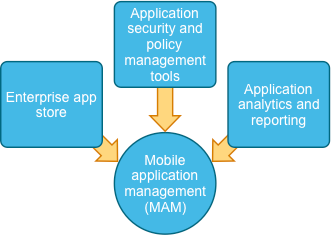
\includegraphics[width=7cm]{img/MAM-Offering}
\caption{Gartner Magic quadrant. Převzato z } 
\label{MAM:nacrt}
\centering
\end{figure}\todo{ citace https://www.ibm.com/developerworks/community/blogs/mobileblog/entry/got\_mam\_mobile\_application\_management\_in\_your\_2013\_mobile\_menu25?lang=en}


\subsection{MCM} 
Mobile content management. Jedná se o software pro správu obsahu na mobilních zařízeních. podle \cite{Gartner_EMM_2016} má tři základní role:
\begin{itemize}
    \item Vynucování politik Dokáže vynutit politiky pro jednotlivé soubory včetně šifrovacích klíčů nezávislých na zařízení, autentifikace, pravidel pro sdílení souborů či pravidel pro copy and paste funkcionalitu.
    \item Přístup k obsahu. Vynutí pravidla pro distribuci, záměnu a mazání souborů.
    \item Integrace Přidává kompaktibilitu pro systémy správy práv, jako jsou ochrana ztráty dat (DLP) nebo podniková správa práv (EDRM) od třetích stran.
\end{itemize}
 
 
 %Vyberte nejvhodnější variantu na trhu dostupného řešení a konfrontujte ji s praxí ve vybrané organizaci. 
\section{Výběr nejvhodnější varianty}

Předchozí analýzy prokázaly, že neexistuje řešení, které by dokázalo zastřešit všechny případy užití vlastních zařízení ve firemním prostředí. Proto tato práce bude dále dělit BYOD podle typu zařízení, a to na mobilní zařízení jako jsou mobilní telefony či tablety a notebooky.

\section{Výběr řešení pro mobilní telefony a tablety}

%\todo{Proc je potreba EMM? Viz specifikace projektu Good}
Podle analýzy \ref{identifikovanePotreby} uživatelé žádají ze svých osobních mobilních telefonů a tabletů přístup k emailům a ke kalendáři. Firma se naopak snaží oddělit firemní data od soukromých tak, aby nad nimi měla kontrolu. Tyto požadavky splňují řešení EMM.  

Trh s nástroji v posledních letech výrazně rostl, zároveň se však konsolidoval \cite{IDC2}. V grafech \ref{EMM:podil2015} a \ref{EMM:podil2016} je patrný nárůst trhu s EMM mezi lety 2014 a 2015 z 1,4 miliardy dolarů na 1,8 miliardy dolarů, tedy o 26,9 \%. Zároveň je vidět zvyšování tržního podílu velkých hráču. Výrazný vliv měla také akvizice společnosti Good Technology společností BlackBerry.

 
\begin{figure}[h!]
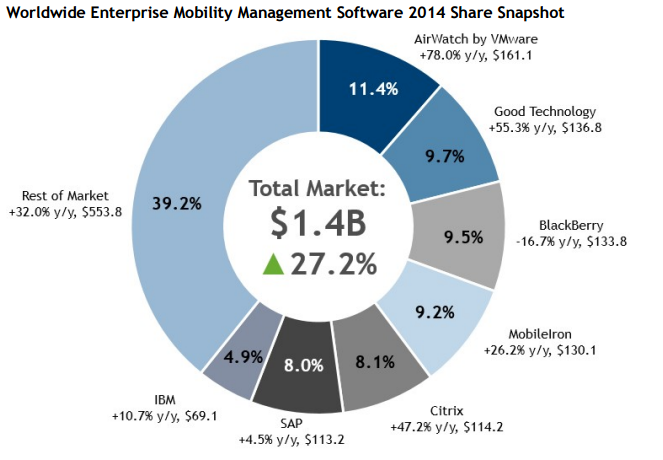
\includegraphics[width=13cm]{img/IDC_EMM}
\caption{Podíl jednotlivých poskytovatelů EMM na trhu v roce 2014 podle IDC. Převzato z \cite{IDC1}.} 
\label{EMM:podil2015}
\centering
\end{figure}

\begin{figure}[h!]
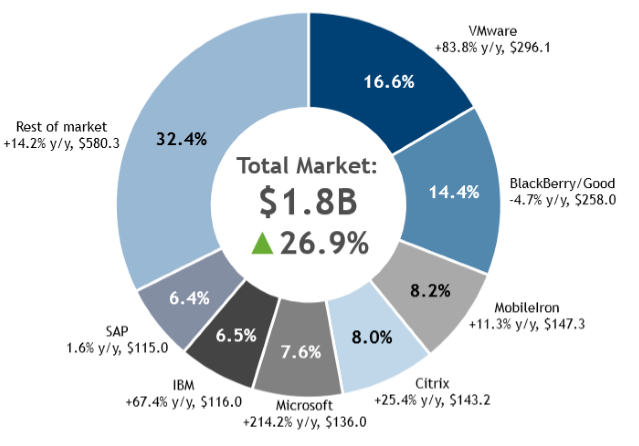
\includegraphics[width=13cm]{img/IDC2016}
\caption{Podíl jednotlivých poskytovatelů EMM na trhu v roce 2015 podle IDC. Převzato z \cite{IDC0}.} 
\label{EMM:podil2016}
\centering
\end{figure}

Podle magazínu CIOReview \cite{CIOReview} bylo v roce 2016 pro BYOD nejslibnějších následujících dvacet poskytovatelů softwaru: Accelion, API Systems, Cyber adAPT, Ericom Software, Excelerate Systems, GSG Telco, High Point Solutions, LANDESK Software,  Mathe, MobileIron, MobilityLab, Movius, RES Software, Sirama Consulting, Skycure, Storgrid, Tangoe, Tyfone, VmWare AirWatch, Zix Corporation.

Některé z nich jsou však příliš úzce zaměřené, či jsou pouze minoritními hráči na trhu. Analýza společnosti Gartner \cite{Gartner_EMM_2016} z roku 2016 pro EMM rozděluje jednotlivé poskytovatele dle jejich postavení na trhu a zároveň hodnotí jejich schopnost zohlednit v produktu aktuální požadavky trhu a nasměrování produktu k budoucím potřebám zákazníků. Tato kritéria shrnuje společnost Gartner jako osy "schopnost vykonat" a "úplnost vize" ve svém grafu nazývaném magic quadrant \ref{EMM:quadrant}.



\begin{figure}[h!]
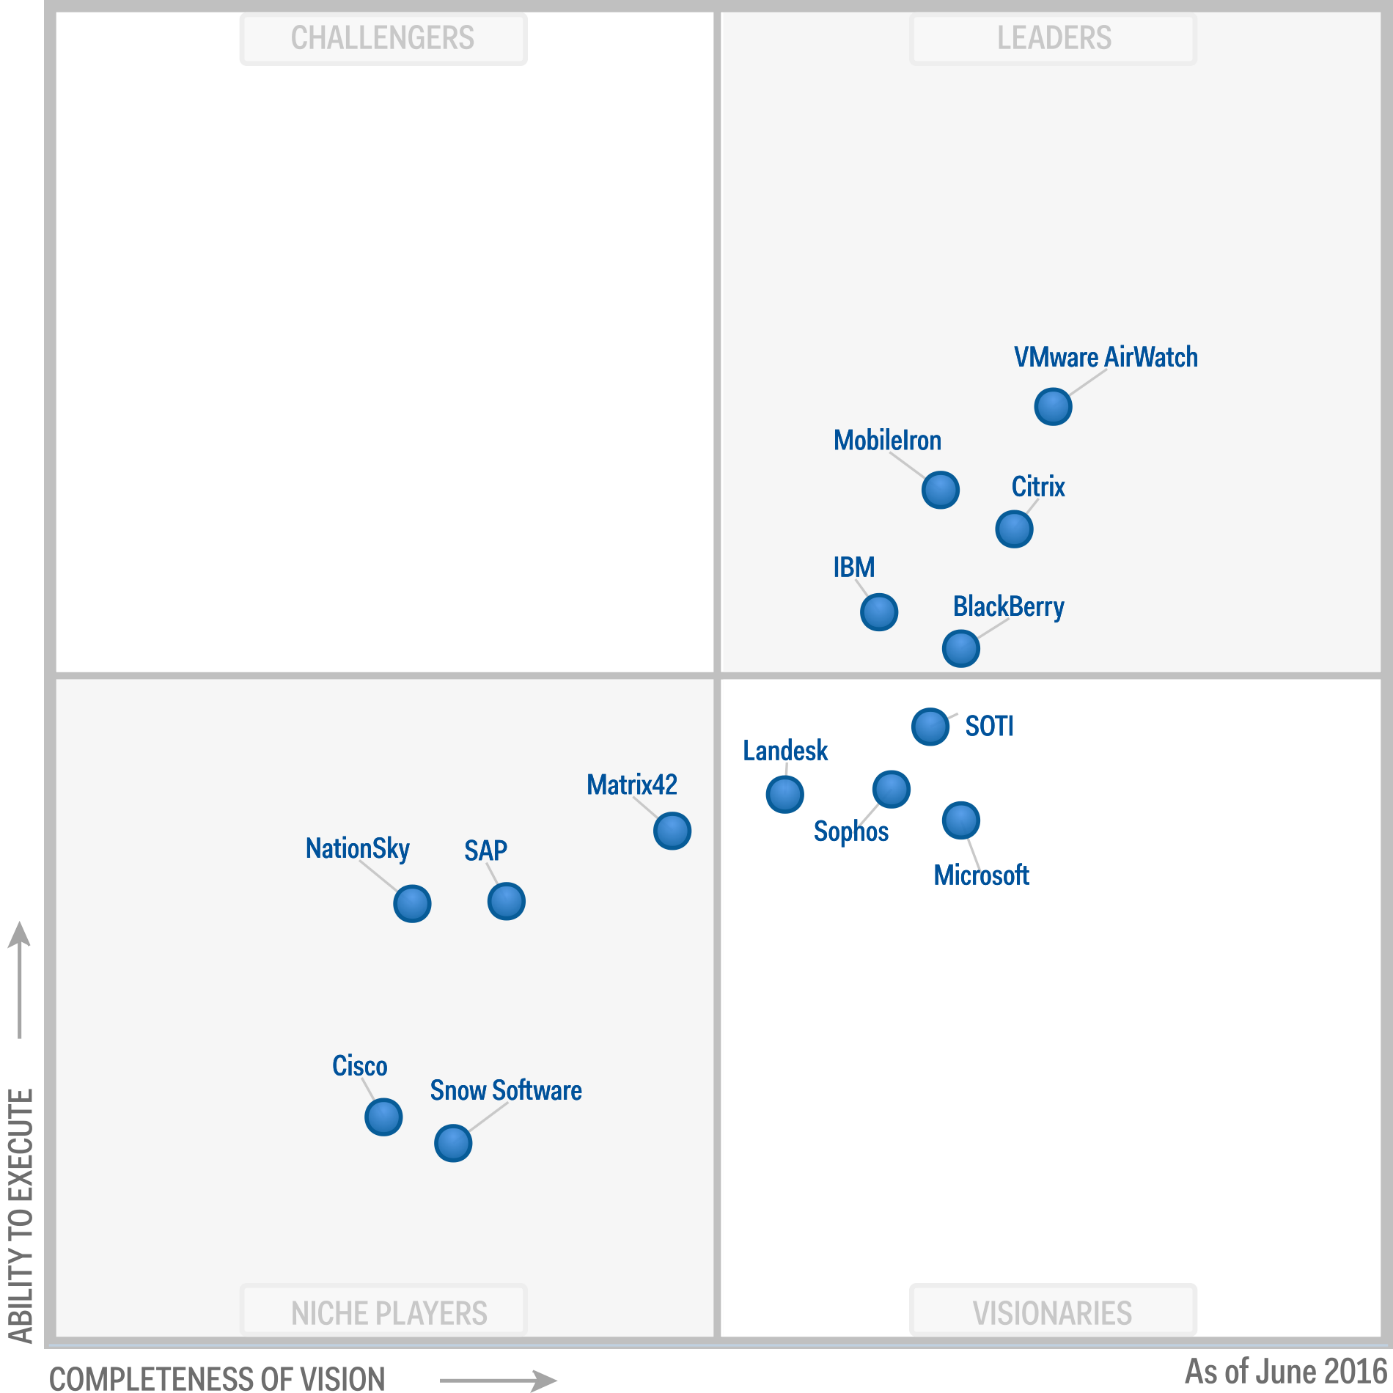
\includegraphics[width=13cm]{img/Gartner_EMM}
\caption{Gartner Magic quadrant. Převzato z \cite{Gartner_EMM_2016}} 
\label{EMM:quadrant}
\centering
\end{figure}
 
Následující společnosti se nacházejí v kvadrantu lídrů:


\subsubsection{VMWare Airwatch}
VMWare koupil společnost AirWatch v roce 2014, viz \cite{VmBuyAir}. Od té doby VMWare zařadil tento EMM do svého porfolia a postupně jej integruje s dalšími produkty jako jsou jeho nástroje pro IAM (Identity and Access Management) a SDN (software-defined networking). AirWatch nabízí širokou podporu pro nástroje třetích stran a je jedním ze zakládajících členů standardu AppConfig. VMWare AirWatch je vhodný pro společnosti, které hledají rozsáhlou funkcionalitu s podporou mnoha platforem.

Podle \cite{Gartner_EMM_2016} byla prokázána nasaditelnost do rozsáhlých prostředí a snadná administrace. Na druhou stranu se objevily problémy s technickou podporou a také nutnost použít řešení od třetí strany pro PIM (Person information management).



\subsubsection{MobileIron}
MobileIron je veřejně obchodovatelná společnost (NASDAQ: MOBL), která se jako jedna z posledních soustředí pouze na svůj EMM produkt. Nabízí však širokou podporu aplikací třetích stran a je jedním ze zakládajících členů standardu AppConfig. Společnost je ceněna pro schopnost přinášet nové funkce na všechny tři hlavní mobilní platformy a plnění amerických bezpečnostních certifikací. Jedná se o produkt, který nabízí mnoho funkcí, škálovatelnost, stabilitu a integraci s dalšími aplikacemi.

Řešení nabízí nástroj pro reporting, pokročilou integraci se SIEM (security information and event management) řešeními třetích stran či správu z mobilního zařízení. Získává kladné ohlasy na svou stabilitu, použitelnost, škálovatelnost a rozsáhlý ekosystém přidružených aplikací AppConnect. MobileIron se drží mezi prvními při nasazování pro nové verze operačních systému.

Na druhou stranu podle \cite{Gartner_EMM_2016} jsou známé případy, kdy zákazníci měli potíže získat technickou podporu. Aplikace Apps@Work nabízejí zastaralý uživatelský zážitek a zároveň existuje nejistota ohledně budoucnosti firmy vzhledem ke změnám ve vrcholném managementu.

\subsubsection{Citrix}
Řešení od společnosti Citrix se skládá z produktů NetScaler, ShareFile a Xen Mobile. Je silné především díky balíku kontejnerizovaných aplikací Worx. ShareFile je kvalitní EFSS (Enterprise file synchronization and sharing) řešení. Obsahuje též uživatelsky přívětivé DLP (Data loss prevention). XenMobile je vhodný pro společnosti s existující infrastrukturou od Citrixu nebo pro ty, jež požadují široké spektrum funkcí.

Společnost Gartner zaznamenala problémy u nasazení XenMobile jako SaaS (Software as a service) u velkých projektů (tj. více než 20000 zařízení) \cite{Gartner_EMM_2016}. Přestože XenMobile nabízí možnost virtualizace Windows aplikací pro mobilní zařízení, použitelnost je na na mobilních zařízeních sporná, vzhledem k dotykové povaze ovládání uživatelského rozhraní. 


\subsubsection{IBM}
IBM nabízí kompletní balík EMM nástrojů MaaS360. Podporuje všechny významné operační systémy, nabízí dobrou spolupráci s dalším bezpečnostním software od IBM. Jedná se o produkt, který má velký záběr, co se týče funkcionality, ale přitom je snadno nasaditelný, viz \cite{Gartner_EMM_2016}.



\subsubsection{BlackBerry}
BlackBerry nyní prodává svůj nástroj jako Good Secure EMM Suite. Skládá se z BES12, Good collaboration apps, Good dynamics a WatchDox Enterprise. Produkty pod značkou Good a WatchDox získala Blacberry akvizicemi které byly dokončeny v roce 2015, viz \cite{BBBuyDox, BBBuyGood}.

Podle agentury Gartner je Good Secure EMM Suite vhodný pro organizace s přísnými požadavky na bezpečnost či působící v regulovaném sektoru. Těm nabízí silnou sadu nástrojů pro ochranu. Zároveň existuje silná podpora pro starší verze software od BlackBerry. Nástroj Good Work nabízí jeden z nejlepších zabezbečených Personal information manager (PIM) nástrojů. Podpora od BlackBerry získává mnoho kladných hodnocení od zákazníků. 

Vícevrstvá cloudová verze produktu BES12 umisťuje data do datacenter ve dvou lokacích, a to Kanadě a Nizozemsku. To by mohl být pro některé bezpečnostní politiky problém. Zároveň u balíku od společnosti BlackBerry dochází k roztříštěnosti služeb mezi jednotlivými produkty.


Další řešení:

\subsubsection{Cisco}
Cisco se dostalo mezi společnosti nabízející MDM software akvizicí společnosti Meraki v roce 2012 \cite{CiscoBuyMeraki}. Kromě řešení pro Android a iOS nabízí také podporu pro Windows a MAC OS X. Nabízí hlubokou integraci do síťové ingrastruktury. Správa produktu nabízí velice jednoduché a přívětivé uživatelské rozhraní. Cenově se jedná o levnější řešení než u většiny konkurentů.

Výhody integrace do síťové infrastruktury je možné využít pouze v případě, že organizace používá sítovou infrastrukturu od Cisco/Meraki. Meraki neobsahuje všechny součásti EMM, soutředí se pouze na MDM.



\subsubsection{Microsoft}
EMM produkt od Microsoftu se nazývá Enterprise Mobility Suite. Skládá se z Microsoft Intune, Azure Active Directory Premium, Advanced Threat Analytics a Azure Rights Management. MDM a MAM služby jsou soustředěny v Microsoft Intune. Toto řešení je nabízeno pouze jako služba v cloudu. Řešení od Microsoftu je vhodné pro společnosti, které nemají vysoké nároky na správu a používají Office 365 nebo Azure Active Directory.

\subsubsection{Landesk}
Landesk se zaměřuje především na UEM (User Evironment Management) a jeho řešení Landesk Mobility Suite tak zapadá do jeho portfolia jako doplněk pro mobilní zařízení. Je tedy vhodné především pro firmy, které mají potřebu spravovat desktopové prostředí a mobilní zařízení zároveň.

\subsubsection{Další řešení}
Ostatní řešení byla v \cite{Gartner_EMM_2016} prezentována jako nabízející příliš úzké zaměření, nedostatečnou funkcionalitu nebo nevhodnost pro nasazení ve větším měřítku


\section{Výběr řešení pro notebooky}

Vzhledem k požadavkům na bezpečnost a dodržování přísných firemních politik v bance a zároveň k potřebě přístupů k různým typům software a aplikací se zdá jako jediné vhodné řešení BYOD virtualizace desktopu. Způsobů, jakými může virtualizace sloužit pro řešení BYOD je více.

Analýza \cite{ForresterWave} ze září roku 2015 od společnosti Forrester se zaměřuje na virtuální desktopy umístěné na vlastním serveru. Výhodou oproti DaaS řešení je, že aplikace i data jsou pod úplnou kontrolou IT oddělení, což snižuje riziko ztráty nebo krádeže dat. Nevýhodou těchto řešení může být problémová funkčnost některých periferních zařízení, jako jsou webové kamery nebo tiskárny. Dále jsou tato řešení velmi citlivá na stabilitu a rychlost internetového připojení, a především u graficky náročnějších aplikací. 

\begin{figure}[h!]
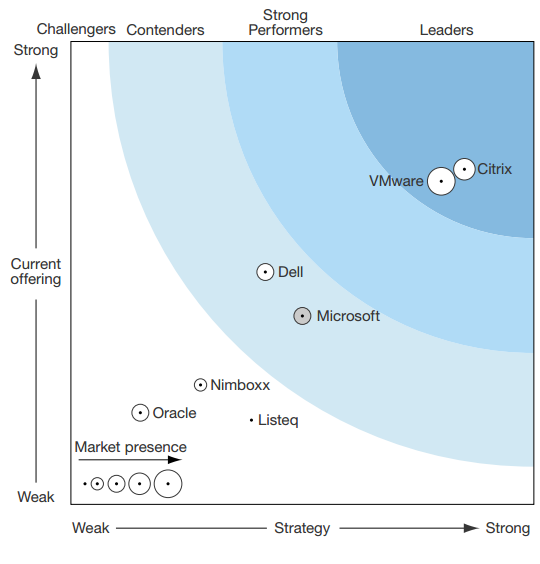
\includegraphics[width=13cm]{img/Forrester_Wave}
\caption{The Forrester Wave: Virtuání desktopy umístěné na serveru. Převzato z: \cite{ForresterWave}.} 
\label{Forrester_Wave}
\centering
\end{figure}

Podle této analýzy jsou jasnými lídry trhu s centralizovanou virtualizací společnosti Citrix a VMWare, a to s obrovským tržním i technologickým náskokem. V grafu \ref{Forrester_Wave} je vidět také společnost Dell, která však již vlastní řešení dále nenabízí a prohlubuje spolupráci s produkty od VMWare, jelikož tuto společnost získala akvizicí jejího původního vlastníka společnosti EMC, v září roku 2016 \cite{DellBuyEMC}.

Průzkum trhu od společnosti IDC \cite{IDCVCC} z roku 2016 má širší zaměření, a to na poskytovatele VCC (Virtual Client Computing). Ty definuje jako poskytovatele, kteří tvoří a prodávají software pro virtualizaci se zaměřením na centralizované virtuální desktopy, distribuované virtuální desktopy a software pro virtuální uživatelské sezení (VUS). Průzkum je zaměřen především na obchodní úspěch hodnocených společností. Dále doporučuje zohlednit při výběru poskytovatele kvalitu systému pro správu zařízení, bezpečnost řešení, možnosti grafického výstupu a kompaktibilitu s užívanými aplikacemi. 

\begin{figure}[h!]
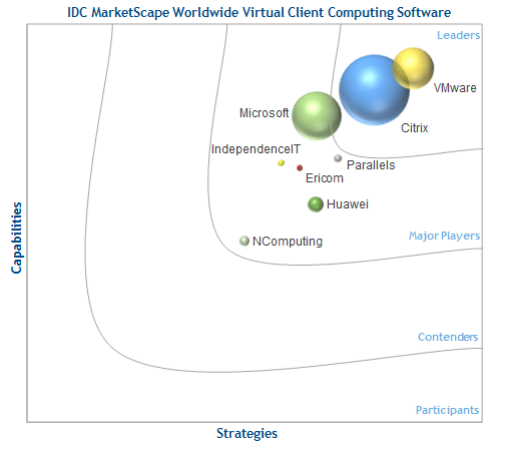
\includegraphics[width=13cm]{img/IDC_VM}
\caption{IDC MarketScape: Hodnocení dodavatelů VCC. Převzato z: \cite{IDCVCC}.} 
\label{IDC_VM}
\centering
\end{figure}

Podle tohoto průzkumu trhu s VCC jasně vládnou společnosti VMWare a Citrix. Nikdo další již nebyl zařazen do segmentu lídrů. Za zmínku dále stojí Microsoft, který má na trhu silnou pozici.



\subsection{Citrix}
Řešení XenDesktop se vyznačuje podporou vlastního protokolu HDX  díky kterému se snaží o adaptivní kompresi, de-duplikaci síťového provozu a přesměrování tíhy renderování dle okolností na klienta a to na všech podporovaných platformách \cite{CitrixHDX}. Dále podporuje vícenásobné 4k monitory a pokročilé funkce pro multimedia a videokonference. Výhodou je podpora amerického bezpečnostního standardu FIPS 140-2.
Podle \cite{ForresterWave} má XenDesktop výborné uživatelské hodnocení, avšak technická podpora je pomalá.

Oproti konkurenčnímu produktu od VMWare nabízí Citrix i virtualizaci Linuxových desktopů. Chlubí se třikrát rychlejším tiskem, šestkrát rychlejším spouštěním aplikací, pětkrát rychlejším ukládání souborů či podporou virtualizovaného Skype for Bussiness. Je možné jej nasadit na jakýkoliv cloud, jakýkoliv hypervizor, síť, do cloudu, lokálně či hybridně, viz \cite{CitrixInfo, CitrixPaper}.

XenDesktop je možné provozovat také v cloudu. Zvolit lze libovolný hypervizor z nabídky VMWare ESX, Microsoft Hyper-V nebo Citrix XenServer. Pro offline použití existuje hypervizor typu 2 pro MacOS a Windows jménem DesktopPlayer. 

Pro virtualizaci aplikací nabízí Citrix platformu XenApp.


\subsection{VMWare}
VMWare nabízí produkt VMWare \textbf{Horizon View}. Použitý protokol je PCoIP od firmy Teradici. Je vhodný v kombinaci serverem vSphere, kdy nabízí dobrou integraci. Nabízí též škálování do cloudu v kooperaci s řešením Horizon Air. Taktéž moduly software od VMWare splňují bezpečnostní standard FIPS 140-2 \cite{VMFIPS}. Horizon View je také možné zakoupit jako součást kompletního balíku, který obsahuje taktéž Horizon Flex pro offline použití. Podle \cite{ForresterWave} hodnotí zákazníci produkt jako dobrý s několika problémy, jako například nutnost použití příkazové řádky pro některá nastavení.

Další produkty pro virtualizaci pracovních prostředí jsou podle výrobce \cite{VMProdukty} následující:


\textbf{Horizon 7} je platforma od VMWare pro virtuální desktopy a aplikace. \textit{Řešení Horizon 7 umožňuje zajišťovat, spravovat a chránit virtuální desktopy (VDI) a aplikace prostřednictvím jedné platformy.}

\textbf{Horizon Air} je DaaS řešení od VMWare. \textit{Poskytuje virtuální desktopy a aplikace hostované v cloudu s širokou škálou možností včetně sdílených desktopů a aplikací.}

\textbf{Horizon Flex} je řešení, které \textit{doručuje, spravuje a zabezpečuje místní virtuální desktopy se systémem Windows na počítačích Mac i PC a současně zajišťuje zabezpečení, možnosti řízení a dodržování požadavků.}

\textbf{App Volumes} je \textit{portfolio integrovaných řešení pro správu aplikací a uživatelů pro virtuální prostředí řešení Horizon, Citrix XenApp a XenDesktop a RDSH.}

\textbf{Mirage} \textit{nabízí správu bitových kopií desktopů pro fyzické desktopy a zařízení POS v nejrůznějších distribuovaných prostředích.}

\textbf{NSX for Horizon} \textit{je síťové řešení infrastruktury virtuálních desktopů (VDI) se zásadami, které jsou dynamicky spojeny s desktopy.}

\textbf{Virtual SAN for Horizon} \textit{Řešení VMware vSAN snižuje zákazníkům počáteční náklady a umožňuje jim využívat celou řadu předkonfigurovaných zařízení pro řešení Horizon, včetně zařízení Virtual SAN Ready Node a infrastruktury postavené na řešení EVO SDDC.}

\textit{VMware \textbf{ThinApp} je řešení pro virtualizaci aplikací bez agentů, které izoluje aplikace od použitých operačních systémů a díky tomu eliminuje konflikty a zjednodušuje doručování a správu.}

\textbf{Řešení User Environment Manager} \textit{nabízí podnikovou správu uživatelů vytvářející přizpůsobené prostředí pro koncové uživatele na všech zařízeních a místech.}

\textbf{Produkty Fusion počítače Mac} \textit{Pomocí řešení VMware Fusion a VMware Fusion je možné používat na počítači Mac bez restartování systém Windows a stovky dalších operačních systémů.}

\textbf{Produkty Workstation systém Windows} Řešení VMware Workstation a VMware Workstation Player představují oborový standard pro používání více operačních systémů jako virtuálních strojů na jednom počítači PC.

\textbf{Řešení Workstation systém Linux} Produkty řešení VMware Workstation systém Linux představují oborový standard pro používání více operačních systémů jako virtuálních strojů na jednom počítači se systémem Linux.

VMware tvrdí, že jeho řešení nabízí oproti konkurenčnímu Citrixu lepší správu a reporting nebo také centrální správu obrazů systémů ať už pro fyzické, virtuální nebo BYOD stroje \cite{VMBetter}. 


\subsection{Microsoft}
Microsoft nabízí virtuální pracovní stanice skrze platformu Windows Server. Nenabízí sice DaaS řešení, ale nabízí virtualizaci aplikací Microsoft Azure RemoteApp. Ty mohou fungovat buďto v čistě cloudovém nebo hybridním módu. VDI je provozováno pod značkou RDS (Remote Desktop Service) jako uživatelské sezení na Windows Server. Z toho důvodu nenabízí tolik možností nastavení a správy jako plná virtualizace \cite{VMwareMicrosoft}.

\subsection{Oracle}
Oracle nabízí nástroj Secure Global Desktop, který je možné použít s různými hypervizory, je ovšem optimalizovaný pro Oracle. Hlavní devízou řešení je kvalitní konzole pro správu Oracle Enterprise Manager. Podle \cite{ForresterWave} toto řešení není vhodné pro případy užití mimo prostředí s vysokým podílem aplikací od Oracle.

Dále nabízí program VirtualBox. Jedná se o hypervizor typu 2, v základní verzi je zdarma i pro komerční užití. Je zaměřený spíše na vývojáře a nenabízí mnoho nástrojů pro vzdálenou správu \cite{OracleVB}.

\subsubsection{Amazon}

Amazon nabízí DaaS službu Amazon Workspaces. Je postavená na platformě Windows server 2008 a používá protokol PCoIP, viz \cite{AmazonAWS}. Je možné volit z mnoha hardwarových konfigurací. Službu lze propojit s firemním Active directory.

\chapter{Návrh řešení}\label{k4}
  %Vyberte nejvhodnější variantu na trhu dostupného řešení a konfrontujte ji s praxí ve vybrané organizaci. 
\section{Výběr nejvhodnější varianty}

Předchozí analýzy prokázaly, že neexistuje řešení, které by dokázalo zastřešit všechny případy užití vlastních zařízení ve firemním prostředí. Proto tato práce bude dále dělit BYOD podle typu zařízení a to na mobilní zařízení jako jsou mobilní telefony či tablety a notebooky.

\section{Výběr řešení pro mobilní telefony a tablety}

\todo{Proc je potreba EMM? Viz specifikace projektu Good}

Trh nástroji v posledních letech výrazně rostl, zároveň se však konsilidoval. \todo{citace https://theictscoop.com/airwatch-consolidates-emm-leadership-in-latest-idc-report-6622602febde   } V grafech \ref{EMM:podil2015} a \ref{EMM:podil2016} je vidět nárůst trhu s EMM mezi lety 2014 a 2015 z 1,4 miliardy dolarů na 1,8 miliardy dolarů, tedy o 26,9 \%. Zároveň je vidět zvyšování tržního podílu velkých hráču. Výrazný vliv měla také akvice společosti Good Technology společností BlackBerry.

 
  \begin{figure}[h]
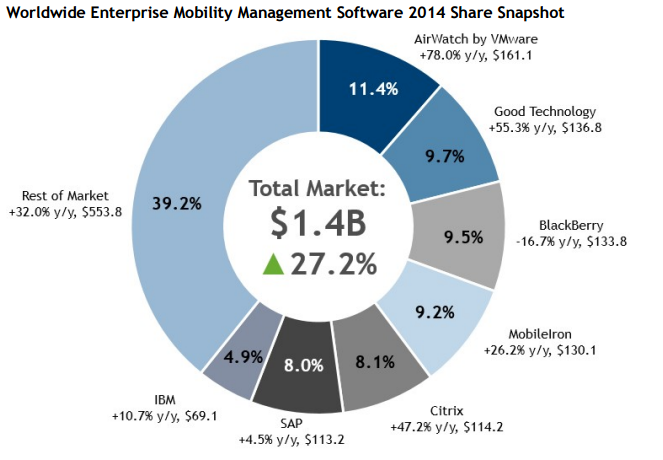
\includegraphics[width=13cm]{img/IDC_EMM}
\caption{Podíl na trhu jednotlivých poskytovatelů EMM v roce 2014 podle IDC Převzato z \cite{}} 
\label{EMM:podil2015}
\centering
\end{figure}\todo{citace http://www.idc.com/getdoc.jsp?containerId=US40430516  }

  \begin{figure}[h]
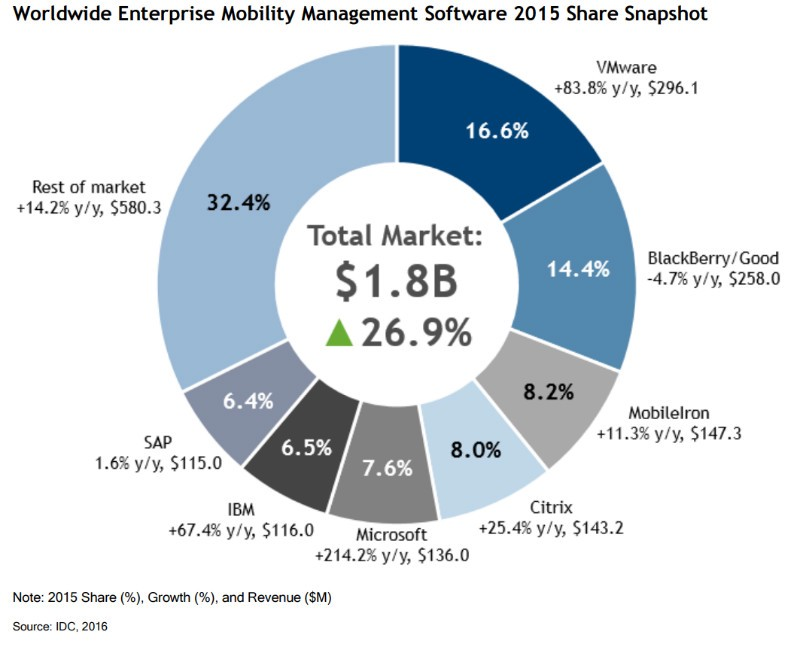
\includegraphics[width=13cm]{img/IDC_EMM_2016}
\caption{Podíl na trhu jednotlivých poskytovatelů EMM v roce 2015 podle IDC Převzato z \cite{}} 
\label{EMM:podil2016}
\centering
\end{figure}\todo{citace https://theictscoop.com/airwatch-consolidates-emm-leadership-in-latest-idc-report-6622602febde   }

Podle magazínu CIOReview bylo v roce 2016 pro BYOD nejslibnějších následujících dvacet poskytovatelů software: Accelion, API Systems, Cyber adAPT, Ericom Software, Excelerate Systems, GSG Telco, High Point Solutions, LANDESK Software,  Mathe, MobileIron, MobilityLab, Movius, RES Software, Sirama Consulting, Skycure, Storgrid, Tangoe, Tyfone, VmWare AirWatch, Zix Corporation.

Některé z nich jsou však příliš úzce zaměřené, či jsou pouze minoritními hráči na trhu. Analýza společnosti Gartner \cite{Gartner_EMM_2016} z roku 2016 pro EMM rozděluje jednotlivé poskytovatele dle jejich postavení na trhu a zároveň zohledňuje jejich schopnost zohlednit v produktu aktuální požadavky trhu a nasměrování produktu k budoucím potřebám zákazníků. Tyto kritéria shrnuje společnost Gartner jako osy "schopnost vykonat" a "úplnost vize" ve svém grafu nazývaném magic quadrant. \ref{EMM:quadrant}



 \begin{figure}[h]
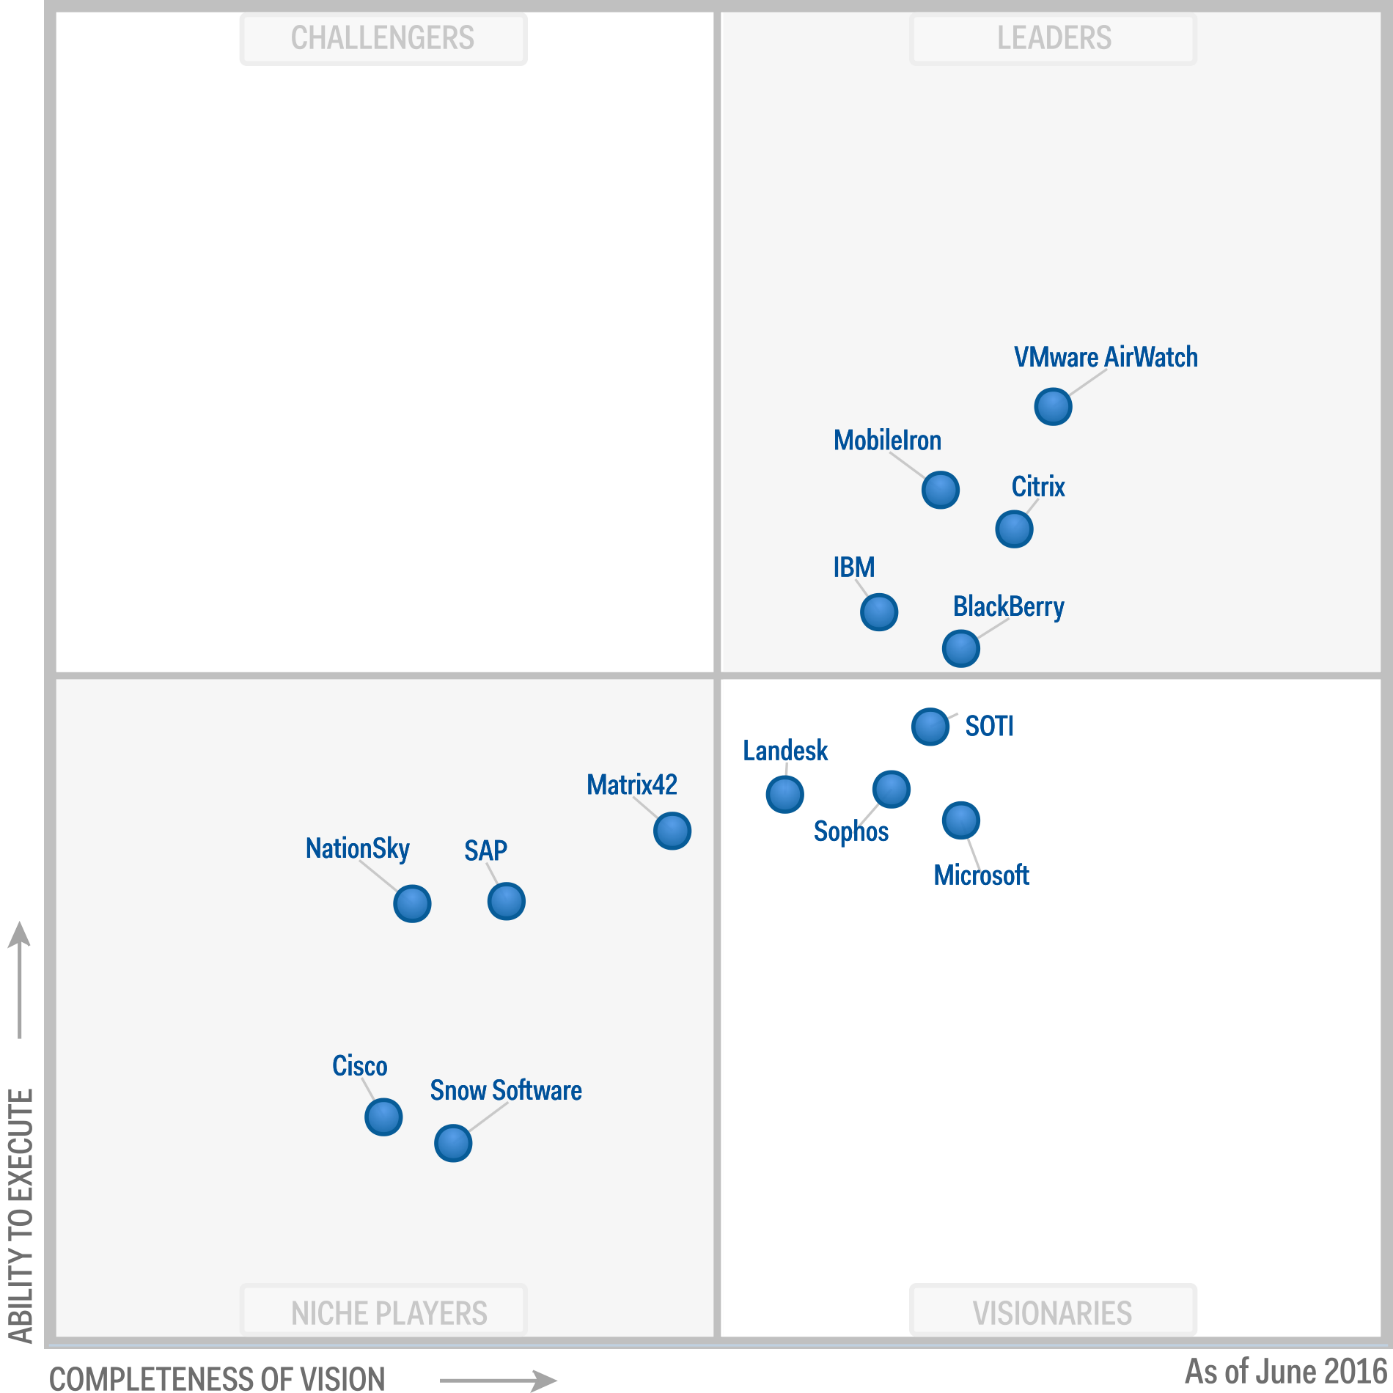
\includegraphics[width=13cm]{img/Gartner_EMM}
\caption{Gartner Magic quadrant. Převzato z \cite{Gartner_EMM_2016}} 
\label{EMM:quadrant}
\centering
\end{figure}\todo{citace}
 %\missingfigure{magic quarter}
 
Následující společnosti se nacházejí v kvadrantu lídrů:


\subsubsection{VMWare Airwatch}
VMWare koupil společnost AirWatch v roce 2014 \todo{citace http://ir.vmware.com/overview/press-releases/press-release-details/2014/VMware-Completes-Acquisition-of-AirWatch/default.aspx}. Od té doby VMWare zařadil tento EMM do svého porfolia a postupně jej integruje s dalšími produkty jakou jsou jeho nástroje pro IAM (Identity and Access Management) a SDN (software-defined networking). AirWatch nabízí širokou podporu pro nástroje třetích stran a je jeden ze zakládajících členů standardu AppConfig. VMWare AirWatch je vhodný pro společnosti, které hledají rozsáhlou funkcionalitu s podporou mnoha platforem.

Podle \todo{citace} byla prokázána nasaditelnost do rozsáhlých prostředí a snadná administrace. Na druhou stranu se objevily problémy s technickou podporou a také nutnost použít řešení od třetí strany pro PIM (Person information management).



\subsubsection{MobileIron}
MobileIron je veřejně obchodovatelná společnost (NASDAQ: MOBL), která jako jedna z posledních soustředí pouze na svůj EMM produkt. Nabízí však širokou podporu aplikací třetích stran a je jedním ze zakládajících členů standardu AppConfig. Společnost je ceněna za schopnost přinášet nové funkce na všechny tři hlavní mobilní platformy a plnění amerických bezpečnostních certifikací. Jedná se o produkt, který nabízí mnoho funkcí, , škálovatelnost, stabilitu a integraci s dalšími aplikacemi.

Řešení nabízí vytváření nástroj pro reporting, pokročilou integraci se SIEM (security information and event management) řešeními třetích stran či správu z mobilního zařízení. Získává kladné ohlasy na svou stabilitu, použitelnost, škálovatelnost a rozsáhlý ekosystém přidružených aplikací AppConnect. MobileIron se drží mezi prvními při nasazování pro nové verze operačních systému.

Na druhou stranu podle \todo{citace} jsou známé případy, kdy zákazníci měli obtíže získat technickou podporu, aplikace Apps@Work nabízejí zastaralý uživatelský zážitek a zároveň existuje nejistota ohledně budoucnosti firmy vzhledem ke změnám ve vrcholém managementu.

\subsubsection{Citrix}
Řešení od společnosti Citrix se skládá z produktů NetScaler, ShareFile a Xen Mobile. Je silné především díky balíku kontejnerizovaných aplikací Worx. ShareFile je kvalitní EFSS (Enterprise file synchronization and sharing) řešení. Obsahuje též uživatelsky přívětivé DLP (Data loss prevention).XenMobile je vhodný pro společnosti s existující infrastrukturou od Citrixu nebo pro ty co požadují široké spektrum funkcí.

Společnost Gartner zaznamenala probléby u nasazení XenMobile jako SaaS (Software as a service) u velkých projektů (tj. více než 20000 zařízení). Přestože XenMobile nabízí možnost virtualizace Windows aplikací pro mobilní zařízení, použitelnost je na na mobilních zařízeních sporná, vzhledem k dotykové povaze ovládání uživatelského rozhraní. 


\subsubsection{IBM}
IBM nabízí komletní malík EMM nástrojů MaaS360. Podporuje všechny významné operační systémy, nabízí dobrou spolupráci s dalším bezpečnostním software od IBM. Jedná se o produkt, který má velký záběr co se týče funkcionality, ale přitom je snadno nasaditelný.



\subsubsection{BlackBerry}
BlackBerry nyní prodává svůj nástroj jako Good Secure EMM Suite. Skládá se z BES12, Good collaboration apps, Good dynamics a WatchDox Enterprise. Produkty pod značkou Good a WatchDox získala Blacberry akvizicemi které byly dokončeny v roce 2015. \todo{citace http://global.blackberry.com/en/company/newsroom/press?id=1998017} \todo{http://global.blackberry.com/en/company/newsroom/press?id=1946553}

Podle agentury Gartner je Good Secure EMM Suite vhodný pro organizace s přísnými požadavky na bezpečnost či působící v regulovaném sektoru. Těm nabízí silnou sadu nástrojů pro ochranu. Zároveň existuje silná podpora pro starší verze software od BlackBerry. Nástroj Good Work nabízí jeden z nejlepších zabezbečených Personal information manager (PIM) nástrojů. Podpora od BlackBerry získává mnoho kladných hodnocení od zákazníků. 

Vícevrstvá cloudová verze produktu BES12 umisťuje data do datacenter ve dvou lokacích a to Kanady a Nizozemí. To by mohl být pro některé bezpečnostní politiky problém. Zároveň u balíku od společnosti BlackBerry dochází k roztříštěnosti služeb mezi jednotlivými produkty.

\todo{funkce a tak}

Další řešení:

\subsubsection{Cisco}
Cisco se dostalo mezi společnosti nabízející MDM software akvizicí společnosti Meraki v roce 2012 \todo{citace https://newsroom.cisco.com/press-release-content?articleId=1118649}. Kromě řešení pro Android a iOS nabízí také podporu pro Windows a MAC OS X. Nabízí hlubokou integraci do síťové ingrastruktury. Správa produktu nabízí velice jednoduché a přívětivé uživatelské rozhraní. Cenově se jedná o levnější řešení než většina konkurence.

Výhody integrace do síťové infrastruktury je možné využít pouze v případě, že organizace používá sítovou infrastrukturu od Cisco/Meraki. Meraki neobsahuje všechny součásti EMM, soutředí se pouze na MDM.



\subsubsection{Microsoft}
EMM produkt od Microsoftu se nazývá Enterprise Mobility Suite. Skládá se z Microsoft Intune, Azure Active Directory Premium, Advanced Threat Analytics a Azure Rights Management. MDM a MAM služby jsou soustředěny v Microsoft Intune. Toto řešení je nabízeno pouze služba v cloudu. Řešení od Microsoftu je vhodné pro společnosti, které nemají vysoké nároky na správu a používají Office 365 nebo Azure Active Directory.

\subsubsection{Landesk}
Landesk se zaměřuje především na UEM (User Evironment Management) a jeho řešení Landesk Mobility Suite tak zapadá do jeho portfolia jako doplněk pro mobilní zařízení. Je tedy vhodné především pro firmy, které mají potřebu spravovat desktopové prostředí a mobilní zařízení zároveň.

\subsubsection{Další řešení}
Ostatní řešení byla v \todo{citace} byla prezentována jako mající příliš úzké zaměření, nedostatečnou funkcionalitu nebo nevhodnost pro nasazení ve větším měřítku


\section{Výběr řešení pro notebooky}

Vzhledem k požadavkům na bezpečnost a dodržování přísných firemních politik v bance a zároveň k potřebě přístupů k různým typům software a aplikací se zdá jako jediné vhodné řešení BYOD virtualizace desktopu. Způsobů, jakými může virtualizace sloužit pro řešení BYOD je více.

Analýza \ref{Forreste_Wave} z září roku 2015 od společnosti Forrester se zaměřuje na virtuální desktopy umístěné na vlastním serveru. Výhodou oproti DaaS řešení je, že aplikace i data jsou pod úplnou kontrolou IT oddělení, což snižuje riziko ztráty nebo krádeže dat. Nevýhodou těchto řešení může být problémová funkčnost některých periferních zařízení, jako jsou webové kamery nebo tiskárny. Dále jsou tato řešení velmi citlivá na stabilitu a rychlost internetového připojení a to především u graficky náročnějších aplikací. 

 \begin{figure}[h]\label{Forrester_Wave}
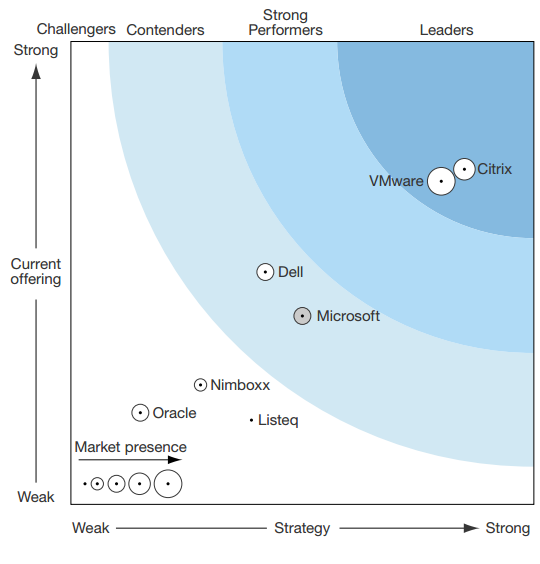
\includegraphics[width=13cm]{img/Forrester_Wave}
\caption{The Forrester Wave: Virtuání desktopy umístěné na serveru} 
\label{EMM:quadrant}
\centering
\end{figure}\todo{citace https://www.citrix.com/content/dam/citrix/en\_us/documents/products-solutions/forrester-wave-server-hosted-virtual-desktops-q3-2015.pdf}

Podle této analýzy jsou jasnými lídry trhu s centralizovanou virtualizací společnosti Citrix a VMWare a to s obrovským tržním i technologickým náskokem. V grafu \ref{Forrester_Wave} je vidět také společnost Dell, která však již vlastní řešení dále nenabízí a prohlubuje spolupráci s produkty od VMWare, jelikož tuto společnost získala akvizicí jejího původního vlastníka, společnosti EMC, v září roku 2016. \todo{citace https://www.emc.com/about/news/press/2016/20160907-01.htm} 

Průzkum trhu od společnosti IDC z roku 2016 \todo{citovat IDC VM} \ref{IDC_VM} má širší zaměření, a to na poskytovatele VCC (Virtual Client Computing). Ty definuje jako poskytovatele kteří tvoří a prodávají software pro virtualizaci se zaměřením na centralizované virtuální desktopy, distribuované virtuální desktopy a software pro virtuální uživatelské sezení (VUS). Průzkum je zaměřen především na obchodní úspěch hodnocených společností. Dále doporučuje zohlednit při výběru poskytovatele kvalitu systému pro správu zařízení, bezpečnost řešení, možnosti grafického výstupu a kompaktibilitu s užívanými aplikacemi. 

 \begin{figure}[h]\label{IDC_VM}
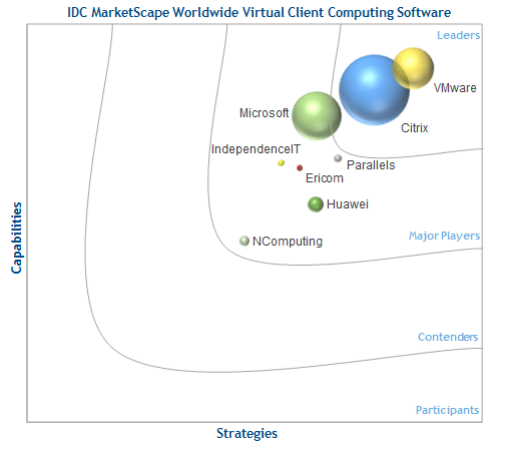
\includegraphics[width=13cm]{img/IDC_VM}
\caption{IDC MarketScape: Hodnocení dodavatelů VCC } 
\label{EMM:quadrant}
\centering
\end{figure}\todo{citace http://campaign.vmware.com/imgs/GlobalCampaigns/39249/IDC\_MarketScape\_Worldwide\_Virtual\_Client\_Computing\_Software\_2016\_Vendor\_Assessment.pdf}

Podle tohoto průzkumu trhu s VCC jasně vládnou společnosti VMWare a Citrix. Nikdo další již nebyl zařazen do segmentu lídrů. Za zmínku dále stojí Microsoft, který má silnou pozici na trhu.



\subsection{Citrix}
Řešení XenDesktop se vyznačuje podporou vlastního protokolu HDX \todo{citace https://www.citrix.com/blogs/2014/08/18/citrix-xendesktopxenapp-what-is-hdx-its-not-just-ica/} díky kterému se snaží o adaptivní kompresi, de-duplikaci síťového provozu a přesměrování tíhy renderování dle okolností na klienta a to na všech podporovaných platformách. Dále podporuje vícenásobné 4k monitory a pokročilé funkce pro multimedia a videokonference. Výhodou je podpora amerického bezpečnostního standardu FIPS 140-2.
Podle \todo{citace forrestera} má XenDesktop výborné uživatelské hodnocení, avšak technická podpora je pomalá.


\subsection{VMWare}
VMWare nabízí produkt VMWare \textbf{Horizon View}. Použitý protokol je PCoIP od firmy Teradici. Je vhodný v kombinaci serverem vSphere, kdy nabízí dobrou integraci. Nabízí též škálování do cloudu v kooperaci s řešením Horizon Air. Taktéž moduly software od VMWare splňují bezpečnostní standard FIPS 140-2. \todo{citace http://www.vmware.com/security/certifications/fips.html}. Horizon View je také možné zakoupit jako součást kompletního balíku, který obsahuje taktéž Horizon Flex pro offline použití. Podle \todo{zase ocitovat forrestera} hodnotí zákazníci produkt jako dobrý s několika problémy, jako například nutnost použití příkazové řádky pro některá nastavení.

Další produkty pro virtualizaci pracovních prostředí jsou podle výrobce \todo{citace http://www.vmware.com/cz/products.html} následující:


\textbf{Horizon 7} je platforma od VMWare pro virtuální desktopy a aplikace. \textit{Řešení Horizon 7 umožňuje zajišťovat, spravovat a chránit virtuální desktopy (VDI) a aplikace prostřednictvím jedné platformy.}

\textbf{Horizon Air} je DaaS řešení od VMWare. \textit{Poskytuje virtuální desktopy a aplikace hostované v cloudu s širokou škálou možností včetně sdílených desktopů a aplikací.}

\textbf{Horizon Flex} je řešení, které \textit{doručuje, spravuje a zabezpečuje místní virtuální desktopy se systémem Windows na počítačích Mac i PC a současně zajišťuje zabezpečení, možnosti řízení a dodržování požadavků.}

\textbf{App Volumes} je \textit{portfolio integrovaných řešení pro správu aplikací a uživatelů pro virtuální prostředí řešení Horizon, Citrix XenApp a XenDesktop a RDSH.}

\textbf{Mirage} \textit{nabízí správu bitových kopií desktopů pro fyzické desktopy a zařízení POS v nejrůznějších distribuovaných prostředích.}

\textbf{NSX for Horizon} \textit{je síťové řešení infrastruktury virtuálních desktopů (VDI) se zásadami, které jsou dynamicky spojeny s desktopy.}

\textbf{Virtual SAN for Horizon} \textit{Řešení VMware vSAN snižuje zákazníkům počáteční náklady a umožňuje jim využívat celou řadu předkonfigurovaných zařízení pro řešení Horizon, včetně zařízení Virtual SAN Ready Node a infrastruktury postavené na řešení EVO SDDC.}

\textit{VMware \textbf{ThinApp} je řešení pro virtualizaci aplikací bez agentů, které izoluje aplikace od použitých operačních systémů a díky tomu eliminuje konflikty a zjednodušuje doručování a správu.}

\textbf{Řešení User Environment Manager} \textit{nabízí podnikovou správu uživatelů vytvářející přizpůsobené prostředí pro koncové uživatele na všech zařízeních a místech.}

\textbf{Produkty Fusion počítače Mac} \textit{Pomocí řešení VMware Fusion a VMware Fusion je možné používat na počítači Mac bez restartování systém Windows a stovky dalších operačních systémů.}

\textbf{Produkty Workstation systém Windows} Řešení VMware Workstation a VMware Workstation Player představují oborový standard pro používání více operačních systémů jako virtuálních strojů na jednom počítači PC.

\textbf{Řešení Workstation systém Linux} Produkty řešení VMware Workstation systém Linux představují oborový standard pro používání více operačních systémů jako virtuálních strojů na jednom počítači se systémem Linux.


\subsection{Microsoft}

\subsection{Oracle}
Oracle nabízí nástroj Secure Global Desktop, který je možné použít s různými hypervizory, je ovšem optimalizovaný pro Oracle. Hlavní devízou řešení je kvalitní konzole pro správu Oracle Enterprise Manager. Podle \todo{zase cituj forestra} toto řešení není vhodné pro případy užití mimo prostředí s vysokým podílem aplikací od Oracle.



%Konzultujte navrhované řešení se zástupci vybrané organizace a stanovte doporučení pro nasazení. 
\section{Hodnocení navrhované varianty zástupci KB}

%Navrhněte nasazení řešení BYOD. 
\section{Návrh řešení}

\todo{vybiram Flex - a proc? http://blogs.gartner.com/mark-lockwood/2014/10/14/is-vmwares-horizon-flex-the-answer-to-byod/}

\todo{Nasazeni - Cisco guide}
\todo{Nasazeni - Cisco Airwatch integration}


%Zhodnoťte uskutečnitelnost řešení a analyzujte benefity a rizika spojená se zavedením navrženého konceptu.
\section{Analýza navrženého řešení}

\chapter{Vyhodnocení}\label{k5}
   %Zhodnoťte uskutečnitelnost řešení a analyzujte benefity a rizika spojená se zavedením navrženého konceptu.
V této kapitole je zhodnocena uskutečnitelnost řešení a analyzovány benefity a rizika spojená se zavedením navrženého konceptu.

\section{Sumarizace navrženého řešení}
Vzhledem k povaze problému, zjištěného analýzou uvnitř společnosti, bylo navrženo zvolit rozdílná řešení podle typu zařízení.

Bylo navrženo postavit koncepci BYOD na třech základních pilířích a to:

\begin{itemize}
    \item Technické řešení pro notebooky
    \item Technické řešení pro mobilní zařízení
    \item Nastavení dalších opatření
\end{itemize}


\section{Uskutečnitelnost navrženého řešení}
%\todo{Zhodnoťte uskutečnitelnost řešení a analyzujte benefity a rizika spojená se zavedením navrženého konceptu}
Z technického hlediska je návrh uskutečnitelný a po odladění technických detailů by z tohoto pohledu nic nebránilo jeho nasazení. Z pohledu obchodního má taktéž smysl, jelikož uskutečněním navržených opatření by se zvýšila bezpečnost informačních a komunikačních systémů zkoumané organizace, přičemž právě vnitřní bezpečnost je vzhledem k jejímu oboru podnikání důležitou součástí korporátní strategie. 

\section{Benefity řešení pro notebooky}

Hlavním benefitem řešení pro BYOD notebooky za použití distribuované virtualizace jsou nízké náklady na nasazení a provoz i vysoká flexibilita. Na rozdíl od centralizované virtualizace s sebou nenese vysoké náklady na úložiště, servery a síťovou infrastrukturu. Stírá známé problémy centralizované virtualizace jako jsou nízká odezva, vysoká citlivost na kvalitu připojení či problémy s provozováním graficky náročných aplikací.

Zároveň však odděluje pracovní prostředí od operačního systému soukromého počítače a zajišťuje tak bezpečnost firemních dat. Velkým benefitem je možnost práce offline při zachování bezpečnosti díky užití virtualizace. Řeší problém s kontraktory a nekontrolovanými zařízeními ve vlastní síti.

Co se týče obecných výhod BYOD, pokud by do programu vstoupilo významné množství zaměstnanců, dá se předpokládat snížení nákladů na IT v rovině snížení nákladů na pořizování firemních zařízení. Dále se dá předpokládat zvýšení spokojenosti u zaměstnanců, kteří by vstoupili do BYOD programu z důvodu nespokojenosti s firemním zařízením. Tyto důvody by však byly pouze vedlejším efektem, hlavním důvodem pro zavedení BYOD programu je nastavení rámce pro existující nefiremní zařízení z důvodu bezpečnosti.

\section{Rizika nasazení navrhovaného řešení pro notebooky}
Největším rizikem nasazení tohoto řešení může být neochota uživatelů přistoupit na tento model, který přináší uživateli nutnost nainstalovat si na své zařízení klientský software a pracovat s ním. U kontraktorů, kteří jsou zaměstnanci partnerských dodavatelských společností, není samozřejmostí povolení virtualizace na jejich pracovních zařízeních a je nutné tuto možnost pro vstup do BYOD programu zajistit.  Dále je třeba individuálně řešit licencování nejrůznějšího softwaru, jelikož není možné v návrhu řešení BYOD programu obsáhnout všechny možné kombinace potřebného software a licenčních politik. Z hlediska bezpečnosti řešení odstraňuje aktuální bezpečnostní hrozby spojené s připojováním nefiremních zařízení. Bezpečnost se tak v tomto ohledu zvyšuje a nebyly identifikovány žádné přidané bezpečnostní hrozby. 

\section{Benefity navrhovaného řešení pro mobilní telefony a tablety}
Hlavní benefit navrženého řešení pro BYOD mobilní telefony a tablety je vůbec možnost využití konceptu BYOD a tím pádem možnost pracovat kdekoliv. To má potenciál zvýšení produktivity a spokojenosti zaměstnanců. Díky zvoleným licencím a typu nasazení uživatele nijak neomezuje v užívání jejich zařízení a nabízí tak vybalancování pracovního a soukromého života. Důvodem k navržení zavedení konkrétního produktu bylo vysoké zaměření na bezpečnost, které je v bankovním prostředí nejvyšší prioritou.

\section{Rizika nasazení navrhovaného řešení pro mobilní telefony a tablety}
Rizikem může být nedůvěra zaměstnanců k firemnímu softwaru, se schopností kontrolovat jejich soukromé zařízení. Reálný provoz také může ukázat u BYOD zařízení snížení výkonu či snížení výdrže na baterii v určitých konfiguracích. To by znamenalo negativní postoj zaměstnanců k BYOD programu a jeho možný neúspěch.

\section{Další dopady realizace projektu}
Procesní změny nutné k zavedení navrhovaného BYOD programu nejsou nikterak závažné a proto nejsou překážkou k realizaci projektu. Díky nastolení programu pro BYOD je možné nabídnout BYOD některým zaměstnancům a považovat to za pracovní benefit.




\begin{conclusion}\label{k6}
	%sem napište závěr Vaší práce
	\missingfigure{Obrázek s kocickou na konec}
\end{conclusion}


\bibliographystyle{csn690}
\bibliography{mybibliographyfile}

\appendix
\chapter{Seznam použitých zkratek}
% \printglossaries
\begin{description}
	%\item[GUI] Graphical user interface
	%\item[XML] Extensible markup language
	\item[BYOD] Bring your own device -- Nefiremní zařízení používané k práci
	\item[IT] Informační technologie
\end{description}

%% % % % % % % % % % % % % % % % % % % % % % % % % % % % 
% % Tuto kapitolu z výsledné práce ODSTRAŇTE.
% % % % % % % % % % % % % % % % % % % % % % % % % % % % 
% 
% \chapter{Návod k~použití této šablony}
% 
% Tento dokument slouží jako základ pro napsání závěrečné práce na Fakultě informačních technologií ČVUT v~Praze.
% 
% \section{Výběr základu}
% 
% Vyberte si šablonu podle druhu práce (bakalářská, diplomová), jazyka (čeština, angličtina) a kódování (ASCII, \mbox{UTF-8}, \mbox{ISO-8859-2} neboli latin2 a nebo \mbox{Windows-1250}). 
% 
% V~české variantě naleznete šablony v~souborech pojmenovaných ve formátu práce\_kódování.tex. Typ může být:
% \begin{description}
% 	\item[BP] bakalářská práce,
% 	\item[DP] diplomová (magisterská) práce.
% \end{description}
% Kódování, ve kterém chcete psát, může být:
% \begin{description}
% 	\item[UTF-8] kódování Unicode,
% 	\item[ISO-8859-2] latin2,
% 	\item[Windows-1250] znaková sada 1250 Windows.
% \end{description}
% V~případě nejistoty ohledně kódování doporučujeme následující postup:
% \begin{enumerate}
% 	\item Otevřete šablony pro kódování UTF-8 v~editoru prostého textu, který chcete pro psaní práce použít -- pokud můžete texty s~diakritikou normálně přečíst, použijte tuto šablonu.
% 	\item V~opačném případě postupujte dále podle toho, jaký operační systém používáte:
% 	\begin{itemize}
% 		\item v~případě Windows použijte šablonu pro kódování \mbox{Windows-1250},
% 		\item jinak zkuste použít šablonu pro kódování \mbox{ISO-8859-2}.
% 	\end{itemize}
% \end{enumerate}
% 
% 
% V~anglické variantě jsou šablony pojmenované podle typu práce, možnosti jsou:
% \begin{description}
% 	\item[bachelors] bakalářská práce,
% 	\item[masters] diplomová (magisterská) práce.
% \end{description}
% 
% \section{Použití šablony}
% 
% Šablona je určena pro zpracování systémem \LaTeXe{}. Text je možné psát v~textovém editoru jako prostý text, lze však také využít specializovaný editor pro \LaTeX{}, např. Kile.
% 
% Pro získání tisknutelného výstupu z~takto vytvořeného souboru použijte příkaz \verb|pdflatex|, kterému předáte cestu k~souboru jako parametr. Vhodný editor pro \LaTeX{} toto udělá za Vás. \verb|pdfcslatex| ani \verb|cslatex| \emph{nebudou} s~těmito šablonami fungovat.
% 
% Více informací o~použití systému \LaTeX{} najdete např. v~\cite{wikilatex}.
% 
% \subsection{Typografie}
% 
% Při psaní dodržujte typografické konvence zvoleného jazyka. České \uv{uvozovky} zapisujte použitím příkazu \verb|\uv|, kterému v~parametru předáte text, jenž má být v~uvozovkách. Anglické otevírací uvozovky se v~\LaTeX{}u zadávají jako dva zpětné apostrofy, uzavírací uvozovky jako dva apostrofy. Často chybně uváděný symbol "{} (palce) nemá s~uvozovkami nic společného.
% 
% Dále je třeba zabránit zalomení řádky mezi některými slovy, v~češtině např. za jednopísmennými předložkami a spojkami (vyjma \uv{a}). To docílíte vložením pružné nezalomitelné mezery -- znakem \texttt{\textasciitilde}. V~tomto případě to není třeba dělat ručně, lze použít program \verb|vlna|.
% 
% Více o~typografii viz \cite{kobltypo}.
% 
% \subsection{Obrázky}
% 
% Pro umožnění vkládání obrázků je vhodné použít balíček \verb|graphicx|, samotné vložení se provede příkazem \verb|\includegraphics|. Takto je možné vkládat obrázky ve formátu PDF, PNG a JPEG jestliže používáte pdf\LaTeX{} nebo ve formátu EPS jestliže používáte \LaTeX{}. Doporučujeme preferovat vektorové obrázky před rastrovými (vyjma fotografií).
% 
% \subsubsection{Získání vhodného formátu}
% 
% Pro získání vektorových formátů PDF nebo EPS z~jiných lze použít některý z~vektorových grafických editorů. Pro převod rastrového obrázku na vektorový lze použít rasterizaci, kterou mnohé editory zvládají (např. Inkscape). Pro konverze lze použít též nástroje pro dávkové zpracování běžně dodávané s~\LaTeX{}em, např. \verb|epstopdf|.
% 
% \subsubsection{Plovoucí prostředí}
% 
% Příkazem \verb|\includegraphics| lze obrázky vkládat přímo, doporučujeme však použít plovoucí prostředí, konkrétně \verb|figure|. Například obrázek \ref{fig:float} byl vložen tímto způsobem. Vůbec přitom nevadí, když je obrázek umístěn jinde, než bylo původně zamýšleno -- je tomu tak hlavně kvůli dodržení typografických konvencí. Namísto vynucování konkrétní pozice obrázku doporučujeme používat odkazování z~textu (dvojice příkazů \verb|\label| a \verb|\ref|).
% 
% \begin{figure}\centering
% 	
\includegraphics[width=0.5\textwidth, angle=30]{cvut-logo-bw}
% 	\caption[Příklad obrázku]{Ukázkový obrázek v~plovoucím prostředí}\label{fig:float}
% \end{figure}
% 
% \subsubsection{Verze obrázků}
% 
% % Gnuplot BW i barevně
% Může se hodit mít více verzí stejného obrázku, např. pro barevný či černobílý tisk a nebo pro prezentaci. S~pomocí některých nástrojů na generování grafiky je to snadné.
% 
% Máte-li například graf vytvořený v programu Gnuplot, můžete jeho černobílou variantu (viz obr. \ref{fig:gnuplot-bw}) vytvořit parametrem \verb|monochrome dashed| příkazu \verb|set term|. Barevnou variantu (viz obr. \ref{fig:gnuplot-col}) vhodnou na prezentace lze vytvořit parametrem \verb|colour solid|.
% 
% \begin{figure}\centering
% 	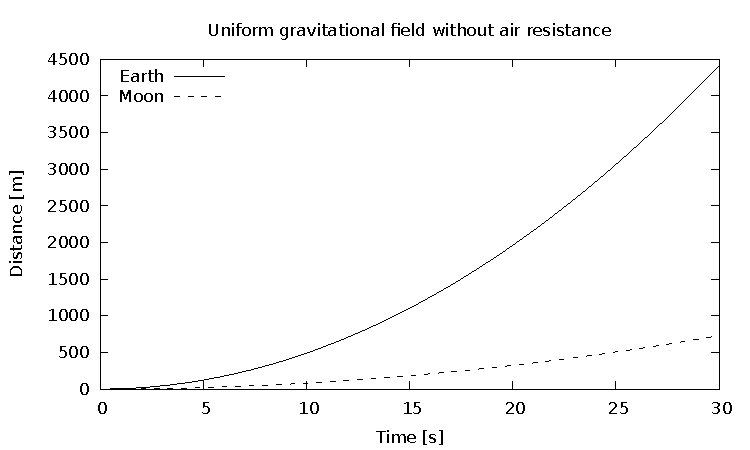
\includegraphics{gnuplot-bw}
% 	\caption{Černobílá varianta obrázku generovaného programem Gnuplot}\label{fig:gnuplot-bw}
% \end{figure}
% 
% \begin{figure}\centering
% 	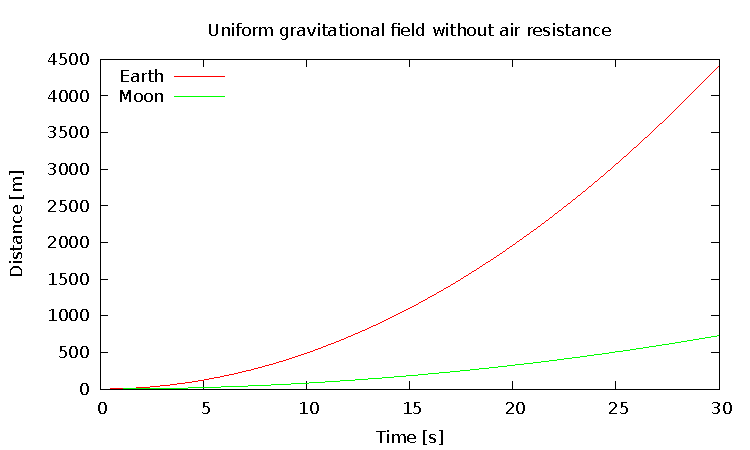
\includegraphics{gnuplot-col}
% 	\caption{Barevná varianta obrázku generovaného programem Gnuplot}\label{fig:gnuplot-col}
% \end{figure}
% 
% 
% \subsection{Tabulky}
% 
% Tabulky lze zadávat různě, např. v~prostředí \verb|tabular|, avšak pro jejich vkládání platí to samé, co pro obrázky -- použijte plovoucí prostředí, v~tomto případě \verb|table|. Například tabulka \ref{tab:matematika} byla vložena tímto způsobem.
% 
% \begin{table}\centering
% 	\caption[Příklad tabulky]{Zadávání matematiky}\label{tab:matematika}
% 	\begin{tabular}{|l|l|c|c|}\hline
% 		Typ		& Prostředí		& \LaTeX{}ovská zkratka	& \TeX{}ovská zkratka	\tabularnewline \hline \hline
% 		Text		& \verb|math|		& \verb|\(...\)|	& \verb|$...$|		\tabularnewline \hline
% 		Displayed	& \verb|displaymath|	& \verb|\[...\]|	& \verb|$$...$$|	\tabularnewline \hline
% 	\end{tabular}
% \end{table}
% 
% % % % % % % % % % % % % % % % % % % % % % % % % % % % 


\chapter{Obsah přiloženého CD}
%upravte podle skutecnosti
 \begin{figure}
	\dirtree{%
		.1 readme.txt\DTcomment{stručný popis obsahu CD}.
		.1 exe\DTcomment{adresář se spustitelnou formou implementace}.
		.1 src.
		.2 impl\DTcomment{zdrojové kódy implementace}.
		.2 thesis\DTcomment{zdrojová forma práce ve formátu \LaTeX{}}.
		.1 text\DTcomment{text práce}.
		.2 thesis.pdf\DTcomment{text práce ve formátu PDF}.
		%.2 thesis.ps\DTcomment{text práce ve formátu PS}.
	}
\end{figure}
 
\chapter{HW požadavky VMware Horizon FLEX}\label{pozadavky}

\section{Horizon FLEX Server}
\begin{itemize}
\item Minimum CPU: 1 Quad-Core Processor or 2 vCPUs
\item 2.26GHz Intel core speed or equivalent
\item Minimum 512MB /Recommended 4GB
\item Disk: 10GB+ /Recommended 40GB+
\item Windows 2008 R2, Windows 2012 and above
\item .NET 3.5 SP1 and above
\item IIS 7.0+ with II6 Management Compatibility and ASP.Net
\end{itemize}

\section{VMware Mirage Server}
\begin{itemize}
\item  Minimum 4 vCPU, Recommended 8 vCPU
\item Minimum 8GB RAM, Recommended 16GB
\item  146GB Free Disk Space
\item Windows 2008 R2, Windows 2012 and above
\item .NET 3.5 SP1 and above
\item IIS 7.0+ with II6 Management Compatibility and ASP.Net 
\end{itemize}




\end{document}
